\documentclass[addpoints]{exam}
\usepackage[utf8]{inputenc}
\usepackage[spanish]{babel}
\usepackage[T1]{fontenc}
\usepackage{charter}
\usepackage{amsmath}
\usepackage{amsfonts}
\usepackage{amssymb}
\usepackage{graphicx}
\usepackage{tikz}
\usetikzlibrary{babel,calc,patterns,decorations.pathmorphing,decorations.markings,arrows.meta,shapes.geometric}
\usepackage{tikz-3dplot}
\usepackage{multicol}
\usepackage{exam-randomizechoices}
\usepackage[left=1cm,right=1cm,top=2cm,bottom=2cm]{geometry}
\usepackage[font=small,labelfont={small,bf},margin=0.5cm,justification=justified]{caption}
\usepackage[font=small,labelfont={small,bf}]{subcaption}
\usepackage[italic,defaultmathsizes]{mathastext}
\usepackage{hyperref}
\usepackage{calculator}
\usepackage[breakable]{tcolorbox}
\usepackage{multirow}
\usepackage{tabularx}
\usepackage{cancel}
\usepackage{tipa}
\usepackage{enumerate}

%\pointpoints{punto}{puntos}
%\bonuspointpoints{punto extra}{puntos extra}

\renewcommand{\solutiontitle}{\textbf{Solución: }}
\renewcommand{\thequestion}{\bfseries\arabic{question}}

\newcommand{\sgn}{\mathop{\mathrm{sgn}}}
\newcommand{\diff}[0]{\mathrm{d}}
\newcommand{\fdiff}[2]{\frac{\mathrm{d} #1}{\mathrm{d} #2}}
\newcommand{\pdiff}[2]{\frac{\partial #1}{\partial #2}}
\newcommand{\fddiff}[2]{\frac{\mathrm{d^2} #1}{\mathrm{d} #2^2}}
\newcommand{\grado}[0]{^{\circ}}
\newcommand{\angulo}[3]{#1\grado \, #2' \, #3''}
\newcommand{\chel}[4]{^{#1}_{#2}\mbox{#3}^{#4}}
\newcommand{\valmed}[1]{\left\langle #1 \right\rangle}
\newcommand{\E}[1]{\times 10^{#1}}
\newcommand{\ver}[1]{\hat{\vec{#1}}}
\newcommand{\vecg}[1]{\boldsymbol{#1}}
\newcommand{\iu}{\mathrm{i}}
\newcommand{\norm}[1]{\left\vert\left\vert #1 \right\vert\right\vert}
\newcommand{\abs}[1]{\left\vert #1 \right\vert}
\newcommand{\tens}[1]{\mathbb{#1}}
\newcommand{\rr}{\mathbb{R}}
\newcommand{\un}[1]{\text{#1}}
\newcommand{\logoUNAHUR}{
\includegraphics[scale=0.35]{/home/shluna/Proyectos/Clases_Fisica_III/imgs/logo_unahur.png}}
\renewcommand{\arraystretch}{1.5}
\newcommand{\rta}{\textbf{Respuesta: }}
\newcommand{\rtas}{\textbf{Respuestas: }}
\newcommand{\ang}{110}
\newcommand{\angu}{-30}
\newcommand{\rad}{4}
\newcommand{\mg}{1}
\newcommand{\muc}{0.5}
\newcommand{\arc}[1]{{%
  \setbox9=\hbox{#1}%
  \ooalign{\resizebox{\wd9}{\height}{\texttoptiebar{\phantom{A}}}\cr#1}}}

\hypersetup{
%      draft,
   linktocpage=true,
    colorlinks=true,
    linkcolor=blue,
    citecolor=blue,
    filecolor=blue,      
    urlcolor=blue
}

\printanswers
\qformat{\textbf{Ejercicio \thequestion}\hfill}

\pagestyle{headandfoot}
\firstpageheader{Instituto de Tecnología e Ingeniería}{\logoUNAHUR}{Física}
\firstpageheadrule
\runningheader{Guía de ejercicios -- Unidad 2}{\logoUNAHUR}{Física}
\runningheadrule
\firstpagefooter{}{Página \thepage\ de \numpages}{}
\firstpagefootrule
\runningfooter{}{Página \thepage\ de \numpages}{}
\runningfootrule

\begin{document}

\renewcommand{\tablename}{Tabla}

\tdplotsetmaincoords{70}{110}

\begin{tcolorbox}[colback=white,arc=0mm,colframe=black]
    \begin{center}
        \Large\textbf{Guía de ejercicios resueltos y propuestos -- Unidad 2}
    \end{center}
\end{tcolorbox}

\vspace{11pt}

\begin{questions}

    \section{Centro de masa}

    \question Calcular las coordenadas del centro de masa del sistema formado por las cuatro masas puntuales indicadas en la Figura~\ref{fig:mxy}.

    \begin{figure}[h]
    \centering
    \begin{tikzpicture}[scale=1]
        \draw[step=1cm,gray,very thin] (-2,-2) grid (4,4);
        \draw[thick,-latex] (-3,0) -- (5,0) node[anchor=north]{$x$ [cm]};
        \draw[thick,-latex] (0,-3) -- (0,5) node[anchor=south]{$y$ [cm]};
        \foreach \x in {-2,-1,1,2,3,4}
        \draw (\x cm,1mm) -- (\x cm,-1mm) node[thick,anchor=north,fill=white] {\scriptsize $\x$};
        \foreach \y in {-2,-1,1,2,3,4}
        \draw (1mm,\y cm) -- (-1mm,\y cm) node[thick,anchor=east,fill=white] {\scriptsize $\y$};
        \draw[fill=black] (-1,1) circle (0.5mm) node[anchor=south]{10 g};
        \draw[fill=black] (1,3) circle (0.5mm) node[anchor=south]{10 g};
        \draw[fill=black] (3,2) circle (0.5mm) node[anchor=south]{20 g};
        \draw[fill=black] (2,0) circle (0.5mm) node[anchor=south]{30 g};
        \draw[fill=black,red] (1.72,1.14) circle (0.5mm) node[anchor=south]{CM};
    \end{tikzpicture}
    \caption{ }
    \label{fig:mxy}
    \end{figure}

    \begin{solution}
    Las coordenadas del centro de masa del sistema representado en la Figura~\ref{fig:mxy} se pueden determinar de forma directa con las expresiones correspondientes:
    \begin{equation*}
        \begin{split}
        x_{\textsc{cm}} &= \frac{\sum\limits_{i=1}^4 m_i \, x_i}{\sum\limits_{i=1}^4 m_i}
                = \frac{m_1 \, x_1 + m_2 \, x_2 + m_3 \, x_3 + m_4 \, x_4}{m_1 + m_2 + m_3 + m_4} \\
                &= \frac{10 \, \text{g} \times (-1 \, \text{cm}) + 10 \, \text{g} \times 1 \, \text{cm} + 20 \, \text{g} \times 3 \, \text{cm} + 30 \, \text{g} \times 2 \, \text{cm}}{10 \, \text{g} + 10 \, \text{g} + 20 \text{g} + 30 \, \text{g}} \\
                & = \frac{120 \, \text{g cm}}{70 \, g}
                = 1.72 \, \text{cm}
        \end{split}
    \end{equation*}
    \begin{equation*}
        \begin{split}
        y_{\textsc{cm}} &= \frac{\sum\limits_{i=1}^4 m_i \, y_i}{\sum\limits_{i=1}^4 m_i}
                = \frac{m_1 \, y_1 + m_2 \, y_2 + m_3 \, y_3 + m_4 \, y_4}{m_1 + m_2 + m_3 + m_4} \\
                &= \frac{10 \, \text{g} \times 1 \, \text{cm} + 10 \, \text{g} \times 3 \, \text{cm} + 20 \, \text{g} \times 2 \, \text{cm} + 30 \, \text{g} \times 0 \, \text{cm}}{10 \, \text{g} + 10 \, \text{g} + 20 \text{g} + 30 \, \text{g}} \\
                & = \frac{80 \, \text{g cm}}{70 \, g}
                = 1.14 \, \text{cm}
        \end{split}
    \end{equation*}
    \end{solution}

    \question Una masa de $2 \, \un{kg}$, está en el punto $(3 \, \text{m}; 0)$ y otra masa de $4 \, \un{kg}$ está en el punto $(6 \, \text{m}; 0)$. Hallar el centro de masa del sistema.

    \rta $x_{\textsc{cm}} = 5$ m; $y_{\textsc{cm}} = 0$.

    \question Tres masas puntuales están situadas en un plano $xy$, del modo siguiente: una masa de $5 \, \un{kg}$ está en el punto $(0; 4 \, \text{m})$, una segunda masa de $1 \, \un{kg}$ está en el punto $(4 \, \text{m}; 0)$ y una última masa de $2 \, \un{kg}$ en el punto $(2 \, \text{m}; 2 \, \text{m})$. Hallar el centro de masa del sistema.

    \rta $x_{\textsc{cm}} = 1$ m; $y_{\textsc{cm}} = 3$ m.

    \section{Dinámica de un sistema de partículas. Cuerpos vinculados}

    \question Dos bloques $A$ y $B$ están unidos por un hilo inextensible y de masa despreciable y se encuentran sobre una superficie horizontal lisa. Sobre el bloque $A$ se aplica una fuerza $\vec{F}$, cuyo módulo es de $50 \, \text{N}$ y forma un ángulo $\varphi = 60\grado$ con el semieje de los $x$ positivos. La masa del bloque $A$ es $m_A = 6 \, \text{kg}$ y la del bloque $B$ es $m_B = 4 \, \text{kg}$.  Hallar la tensión del hilo que une a los bloques y la aceleración del sistema. \label{ej:vinculados1}

    \begin{figure}[h]
        \centering
        \begin{subfigure}{\textwidth}
            \centering
            \begin{tikzpicture}[scale=1]
                \fill[pattern=north east lines] (-3,0) -- (-3,-0.2) -- (4,-0.2) -- (4,0) -- cycle;
                \draw[thick] (-3,0) -- (4,0);
                \draw[thick] (-1,0.5) -- (1,0.5);
                \draw[fill=gray!40] (1,0) rectangle (2,1);
                \draw[fill=gray!40] (-2,0) rectangle (-1,1);
                \node at (1.5,0.5) {$A$};
                \node at (-1.5,0.5) {$B$}; 
                \draw[thick,-latex] (2,0.5) -- ({2*cos(30)+2},1.5) node[anchor=south]{$\vec{F}$};
                \draw[dashed] (2,0.5) -- ({2*cos(30)+2},0.5);
                \draw (3,0.5) arc (0:30:1);
                \node[anchor=south west] at (3,0.5) {$\varphi$};
            \end{tikzpicture}
            \caption{Esquema del Ejercicio~\ref{ej:vinculados1}.}
            \label{fig:vinculados3_esq}
        \end{subfigure}
        \\
        \begin{subfigure}{0.45\textwidth}
            \centering
            \begin{tikzpicture}[scale=1]
                \draw[thick,-latex] (-2,0) -- (2,0) node[anchor=north]{$x$};
                \draw[thick,-latex] (0,-2) -- (0,2) node[anchor=east]{$y$};
                \draw[thick,-latex,black!40!green] (0,0) -- (1.5,0) node[anchor=south]{$\vec{T}$};
                \draw[thick,-latex,red] (0,0) -- (0,-1.5) node[anchor=west]{$\vec{F}_\text{g}^{(B)}$};
                \draw[thick,-latex,blue] (0,0) -- (0,1.5) node[anchor=east]{$\vec{F}_\text{N}^{(B)}$};
                \fill[black] (0,0) circle (0.5mm);
            \end{tikzpicture}
            \caption{Diagrama de cuerpo libre del bloque $B$.}
            \label{fig:vinculados3_DCLB}
        \end{subfigure}
        ~
        \begin{subfigure}{0.45\textwidth}
            \centering
            \begin{tikzpicture}[scale=1]
                \draw[thick,-latex] (-2,0) -- (2,0) node[anchor=north]{$x$};
                \draw[thick,-latex] (0,-2) -- (0,2) node[anchor=east]{$y$};
                \draw[thick,-latex] (0,0) -- (30:2) node[anchor=south east]{$\vec{F}$};
                \draw (1,0) arc (0:30:1);
                \node[anchor=south west] at (1,0) {$\varphi$};
                \draw[thick,-latex,black!40!green] (0,0) -- (-1.5,0) node[anchor=south]{$\vec{T}$};
                \draw[thick,-latex,red] (0,0) -- (0,-1.5) node[anchor=west]{$\vec{F}_\text{g}^{(A)}$};
                \draw[thick,-latex,blue] (0,0) -- (0,1.5) node[anchor=east]{$\vec{F}_\text{N}^{(A)}$};
                \fill[black] (0,0) circle (0.5mm);
            \end{tikzpicture}
            \caption{Diagrama de cuerpo libre del bloque $A$.}
            \label{fig:vinculados3_DCLA}
        \end{subfigure}
        \caption{}
        \label{fig:vinculados3}
    \end{figure}

    \begin{solution}
        Para resolver este ejercicio, debemos aislar cada cuerpo e identificar las fuerzas que actúan sobre cada uno de ellos y realizar los correspondientes diagramas de cuerpo libre, tal como se muestra en las Figuras~\ref{fig:vinculados3} (\subref{fig:vinculados3_DCLA}) y \ref{fig:vinculados3} (\subref{fig:vinculados3_DCLB}).

        Las fuerzas que actúan sobre el bloque $A$ son la tensión del hilo, la fuerza $\vec{F}$ aplicada, su propio peso y la reacción normal de la superficie. Las componentes de dichas fuerzas en el sistema de referencia considerado en la Figura~\ref{fig:vinculados3} (\subref{fig:vinculados3_DCLA}) son:
        \begin{itemize}
            \item $\vec{F} = \left(F \cos \varphi; F \sen \varphi\right)$,
            \item $\vec{F}_\text{N}^{(A)} = \left(0; F_\text{N}^{(A)}\right)$,
            \item $\vec{F}_\text{g}^{(A)} = \left(0; - m_A \, g\right)$,
            \item $\vec{T} = \left(-T;0\right)$.
        \end{itemize} Las componentes $x$ e $y$ de la resultante son:
        \begin{align}
            R_x &= \sum f_x = F \cos \varphi - T = m_A \, a_x, \label{ec:sumfxA} \\
            R_y &= \sum f_y = F \sen \varphi + F_\text{N}^{(A)} - m_A \, g = 0. \label{ec:sumfyA}
        \end{align} Dado que el bloque no se mueve en la dirección vertical, $R_y$ debe ser igual a cero. En cambio, como el bloque se va a acelerar en la dirección horizontal, en virtud de la segunda ley de Newton se tiene que $R_x = m_A \, a_x$, donde $a_x$ es la componente $x$ de la aceleración del sistema.

        Podríamos determinar el módulo de la reacción normal del plano usando la Ecuación~\eqref{ec:sumfyA}, pero no es un dato relevante para este ejercicio.
        
        Las fuerzas que actúan sobre el bloque $B$ son las mismas que aquellas aplicadas al bloque $A$, excepto la fuerza $\vec{F}$. Las componentes de estas fuerzas, para el caso del bloque $B$, en el sistema de referencia considerado en la Figura~\ref{fig:vinculados3} (\subref{fig:vinculados3_DCLB}) son:
        \begin{itemize}
            \item $\vec{F}_\text{N}^{(B)} = \left(0; F_\text{N}^{(B)}\right)$,
            \item $\vec{F}_\text{g}^{(B)} = \left(0; - m_B \, g\right)$,
            \item $\vec{T} = \left(T;0\right)$.
        \end{itemize} Las componentes de la fuerza resultante que actúa sobre el bloque $B$ son:
        \begin{align}
            R_x &= \sum f_x = T = m_B \, a_x, \label{ec:sumfxB} \\
            R_y &= \sum f_y = F_\text{N}^{(B)} - m_B \, g = 0. \label{ec:sumfyB}
        \end{align} Como el bloque $B$ tampoco se mueve en la dirección vertical, la componente $y$ de la resultante debe ser también igual a cero y, en consecuencia, podríamos determinar $F_\text{N}^{(B)}$ de la Ecuación~\eqref{ec:sumfyB}, pero tampoco es un dato relevante para el ejercicio.

        Al igual que ocurre con el bloque $A$, la componente $x$ de la resultante de las fuerzas aplicadas al bloque $B$ también es igual al producto de la masa del bloque $B$ por la aceleración del sistema, tal como se indica en la Ecuación~\eqref{ec:sumfxB}.

        Podemos observar que las Ecuaciones~\eqref{ec:sumfxA} y \eqref{ec:sumfxB} forman un sistema de dos ecuaciones lineales con dos incógnitas ($T$ y $a_x$):
        \begin{align}
            F \cos \varphi - T &= m_A \, a_x, \label{ec:RxA} \\
                            T &= m_B \, a_x, \label{ec:RxB}
        \end{align} Este sistema se puede resolver por cualquiera de los métodos conocidos. Teniendo en cuenta que el módulo de la tensión del hilo aparece sumando en la Ecuación~\eqref{ec:RxB} y restando en la Ecuación~\eqref{ec:RxA}, podemos sumar las dos ecuaciones, con lo cual: $$ F \cos \varphi - T + T = m_A \, a_x + m_B \, a$$ O bien: $$ F \cos \varphi = \left(m_A + m_B\right) a_x$$ De donde se obtiene: $$a_x = \frac{F \cos \varphi}{\left(m_A + m_B\right)}$$ Reemplazando los valores correspondientes, obtenemos: $$ a_x = \frac{50 \, \text{N} \times \cos 60\grado}{\left(6 \, \text{kg} + 4 \, \text{kg}\right)} = 2.5 \, \frac{\text{m}}{\text{s}^2}$$ Una vez determinada la aceleración del sistema, podemos calcular la tensión del hilo usando la Ecuación~\eqref{ec:RxA} o la Ecuación~\eqref{ec:RxB}, cualquiera de las dos nos debe llevar al mismo resultado. Si utilizamos la Ecuación~\eqref{ec:RxB}, tenemos: $$T = 4 \, \text{kg} \times 2.5 \, \frac{\text{m}}{\text{s}^2} = 10 \, \text{N}$$

    \end{solution}

    \question Un bloque de masa $m_1 = 8 \, \text{kg}$ y otro de masa $m_2 = 16 \, \text{kg}$ (Figura~\ref{fig:vinculados1}) se encuentran sobre una superficie horizontal, sin rozamiento, unidos por una cuerda $A$, y son arrastrados hacia la derecha sobre la superficie por una segunda cuerda $B$, adquiriendo una aceleración constante cuyo módulo es de $0.5 \, \frac{\text{m}}{\text{s}^2}$. Calcular la tensión de cada cuerda. \label{ej:vinculados2}

    \begin{figure}[h]
        \centering
        \begin{tikzpicture}[scale=1]
            \fill[pattern=north east lines] (-3,0) -- (-3,-0.2) -- (4,-0.2) -- (4,0) -- cycle;
            \draw[thick] (-3,0) -- (4,0);
            \draw[thick] (-1,0.5) -- node[anchor=south]{$A$} (1,0.5);
            \draw[fill=gray!40] (1,0) rectangle (2,1);
            \draw[fill=gray!40] (-2,0) rectangle (-1,1);
            \node at (1.5,0.5) {$m_2$};
            \node at (-1.5,0.5) {$m_1$}; 
            \draw[thick,-latex] (2,0.5) -- node[anchor=south]{$B$} (4,0.5) node[anchor=south]{$\vec{T}_B$};
            \draw[thick,-latex] (-0.5,1.5) -- node[anchor=south]{$\vec{a}$} (0.5,1.5);
        \end{tikzpicture}
        \caption{ }
        \label{fig:vinculados1}
    \end{figure}

    \begin{solution}
        Aislemos cada cuerpo como se indica por las líneas de puntos, y realicemos los correspondientes diagramas de cuerpo libre para cada uno. Representemos por $T_A$ y $T_B$ las tensiones de las cuerdas $A$ y $B$, respectivamente. El sistema de fuerzas que actúa sobre el bloque de 8 kg está formado por su peso, $\vec{F}_\text{g}^{(1)}$, la reacción normal, $\vec{F}_{\text{N}}^{(1)}$, de la superficie sobre él y la tensión, $\vec{T}_A$, dirigida hacia la derecha. El sistema de fuerzas que actúa sobre el bloque de 16 kg está formado por su peso, $\vec{F}_\text{g}^{(2)}$, la fuerza normal, $\vec{F}_{\text{N}}^{(2)}$, la tensión $\vec{T}_A$, dirigida hacia la izquierda, y la tensión $\vec{T}_B$ dirigida hacia la derecha. 
        
        Si para cada bloque elegimos un sistema de referencia cuyo eje $x$ sea paralelo a la superficie y su eje $y$ sea perpendicular a la misma, entonces las componentes de las fuerzas que actúan sobre el bloque de 8 kg son:
        \begin{itemize}
            \item $\vec{F}_\text{g}^{(1)} = \left(0; - m_1 \, g\right)$, donde $m_1 = 8$ kg;
            \item $\vec{F}_{\text{N}}^{(1)} = \left(0;F_{\text{N}}^{(1)}\right)$;
            \item $\vec{T}_A = \left(T_A; 0\right)$.
        \end{itemize}
        La sumatoria de las componentes verticales de las fuerzas es: $$\sum f_y = F_{\text{N}}^{(1)} - m_1 \, g = 0$$ la cual es igual cero porque el bloque está en equilibrio en la dirección vertical. Se obtiene entonces que $$ F_{\text{N}}^{(1)} = m_1 \, g = 8 \, \text{kg} \times 9.8 \, \frac{\text{m}}{\text{s}^2} = 78.4 \, \text{N}$$ Por otro lado, la sumatoria de las componentes $x$ de las fuerzas que actúan sobre el bloque de 8 kg es: $$\sum f_x = T_A = m_1 \, a$$ donde $a = 0.5 \, \frac{\text{m}}{\text{s}^2}$. En este caso, debemos aplicar la segunda ley de Newton porque el bloque \emph{no} está en equilibrio en la dirección horizontal. De esta última ecuación, obtenemos: $$T_A = 8 \, \text{kg} \times 0.5 \, \frac{\text{m}}{\text{s}^2} = 4 \, \text{N}$$

        Las componentes de las fuerzas que actúan sobre el bloque de 16 kg son:
        \begin{itemize}
            \item $\vec{F}_\text{g}^{(2)} = \left(0; - m_2 \, g\right)$, donde $m_2 = 16$ kg;
            \item $\vec{F}_{\text{N}}^{(2)} = \left(0;F_{\text{N}}^{(2)}\right)$;
            \item $\vec{T}_A = \left(-T_A; 0\right)$;
            \item $\vec{T}_B = \left(T_B; 0\right)$.
        \end{itemize}
        Análogamente al caso anterior, la sumatoria de fuerzas en la dirección vertical debe ser igual a cero dado que este bloque también está en equilibrio en esa dirección: $$\sum f_y = F_{\text{N}}^{(2)} - m_2 \, g = 0,$$ de donde se obtiene: $$F_{\text{N}}^{(2)} = m_2 \, g = 16 \, \text{kg} \times 9.8 \, \frac{\text{m}}{\text{s}^2} = 156.8 \, \text{N}$$ En cambio, la sumatoria de las componentes en la dirección horizontal es: $$ \sum f_x = T_B - T_A = m_2 \, a$$ La cuerda $A$ sirve simplemente para transmitir la fuerza de un bloque a otro, de modo que las fuerzas designadas por $\vec{T}_A$ constituyen un par de acción y reacción, y son numéricamente iguales. Entonces, obtenemos: $$T_B = T_A + m_2 \, a = 4 \, \text{N} + 16 \, \text{kg} \times 0.5 \, \frac{\text{m}}{\text{s}^2} = 12 \, \text{N}$$
    \end{solution}

    \question Dos bloques $A$ y $B$ están unidos mediante una cuerda flexible e inextensible de masa despreciable que pasa por una polea de masa también despreciable. El bloque $A$ está apoyado sobre una superficie horizontal, mientras que el bloque $B$ cuelga suspendido de la cuerda, tal como se muestra en la Figura~\ref{fig:vinculados2}. La masa del bloque $A$ es de 16 kg, mientras que la masa del bloque $B$ es de 8 kg. Despreciando todas las fuerzas de rozamiento e inercia de la polea, hallar la aceleración y la tensión de la cuerda.

    \begin{figure}[h]
        \centering
        \begin{tikzpicture}[scale=1]
            \fill[pattern=north east lines] (-5,-0.25) -- (-0.5,-0.25) -- (-0.5,-3.5) -- (-0.7,-3.5) -- (-0.7,-0.45) -- (-5,-0.45) -- cycle;
            \draw (0,0) circle (0.25cm);
            \draw (-3,0.25) -- (0,0.25);
            \draw (0.25,0) -- (0.25,-2);
            \draw[fill=gray!40] (-3,-0.25) -- (-3,0.75) -- (-4,0.75) -- (-4,-0.25) -- cycle;
            \draw[fill=gray!40] (0,-2) -- (0.5,-2) -- (0.5,-2.5) -- (0,-2.5) -- cycle;
            \draw[thick] (-5,-0.25) -- (-0.5,-0.25) -- (-0.5,-3.5);
            \node at (-3.5,0.25) {$A$};
            \node at (0.25,-2.25) {$B$};
            \draw[thick] (-0.5,-0.25) -- (0,0);
            \draw[fill=black] (0,0) circle (0.5mm);
        \end{tikzpicture}
        \caption{ }
        \label{fig:vinculados2}
    \end{figure}

    \begin{solution}
        Aislemos las dos partes, como se indica por las líneas de puntos. El único efecto de la polea es cambiar la dirección de a cuerda, la cual tira con la misma fuerza $\vec{T}$ de cada bloque.

        Entonces, el sistema de fuerzas que actúa sobre el bloque de 16 kg son su peso, $\vec{F}_\text{g}^{(A)}$, la reacción normal de la superficie, $\vec{F}_\text{N}$, y la tensión de la cuerda, $\vec{T}$. Por otro lado, las fuerzas que actúan sobre el bloque de 8 kg son su peso, $\vec{F}_\text{g}^{(B)}$ y la tensión de la cuerda, $\vec{T}$.

        Si para el bloque $A$ definimos un sistema de referencia cuyo eje $x$ sea paralelo a la superficie horizontal y cuyo eje $y$ sea perpendicular a la misma, entonces las componentes de las fuerzas que actúan sobre el bloque de 16 kg son:
        \begin{itemize}
            \item $\vec{F}_\text{g}^{(A)} = \left(0; - m_A \, g\right)$, donde $m_A = 16$ kg;
            \item $\vec{F}_\text{N} = \left(0; F_\text{N}\right)$;
            \item $\vec{T} = \left(T;0\right)$.
        \end{itemize}
        La sumatoria de las componentes de las fuerzas en la dirección vertical deber ser igual a cero porque el bloque se encuentra en equilibrio en esa dirección: $$R_y^{(A)} = F_\text{N} - m_A \, g = 0,$$ de donde se obtiene: $$F_\text{N} = m_A \, g = 16 \, \text{kg} \times 9.8 \, \frac{\text{m}}{\text{s}^2} = 156.8 \, \text{N}$$ Por otro lado, la sumatoria de fuerzas en la dirección horizontal es distinta de cero porque no existe fuerza alguna que equilibre la acción de la fuerza $\vec{T}$, entonces: 
        \begin{equation}
            \label{ec:RxA_vinculados2}
            R_x^{(A)} = T = m_A \, a_x
        \end{equation} donde $a_x$ es la componente $x$ de la aceleración del sistema.

        Si para el bloque $B$ elegimos un sistema de referencia cuyo eje $x$ tenga dirección vertical, y se considera positivo el sentido hacia abajo, las componentes de las fuerzas que actúan sobre el bloque que cuelga de la cuerda son:
        \begin{itemize}
            \item $\vec{F}_\text{g}^{(B)} = \left( m_B \, g; 0\right)$, donde $m_B = 8$ kg;
            \item $\vec{T} = (-T;0)$.
        \end{itemize}
        Así, la sumatoria de fuerzas en la dirección vertical resulta: 
        \begin{equation}
            \label{ec:RxB_vinculados2}
            R_x^{(B)} =  - T + m_B \, g = m_B \, a_x
        \end{equation} De esta forma, reuniendo las Ecuaciones~\eqref{ec:RxA_vinculados2} y \eqref{ec:RxB_vinculados2}, obtenemos un sistema de dos ecuaciones con dos incógnitas:
        \begin{align*}
                    T &= m_A \, a_x \\
            - T + m_B \, g &= m_B \, a_x,
        \end{align*} del cual obtenemos como resultado que: $T = 52.27 \, \text{N}$ y $a_x = 3.27 \, \frac{\text{m}}{\text{s}^2}$.
    \end{solution}

    \question El bloque $A$ de la Figura~\ref{fig:vinculados2} tiene una masa de $12 \, \un{kg}$ y se mueve sobre una superficie horizontal lisa unido por una cuerda ligera flexible e inextensible, que pasa por una pequeña polea sin rozamiento, a un segundo bloque $B$ suspendido que tiene una masa de $4 \, \un{kg}$.

    \begin{parts}
        \part ¿Cuál es la aceleración del sistema y cuál es la tensión de la cuerda que une ambos bloques?
        \part ¿Cuál será la aceleración del sistema y cuál es la tensión de la cuerda que une ambos bloques si el coeficiente cinético de rozamiento es $0.2$ y se le da al bloque $A$ un ligero empujón hacia la derecha?
    \end{parts}

    \rtas
    \begin{enumerate}[a)]
        \item $a = 2.45 \, \frac{\text{m}}{\text{s}^2}$. $T = 29.4 \, \text{N}$.
        \item $a = 0.98 \, \frac{\text{m}}{\text{s}^2}$. $T = 35.28 \, \text{N}$.
    \end{enumerate}

    \question En la Figura~\ref{fig:ej18}, un bloque $A$, que tiene una masa de $20 \, \un{kg}$, se encuentra en reposo sobre una superficie horizontal unido por una cuerda ligera flexible e inextensible, que pasa por una pequeña polea sin rozamiento, a un balde ($B$) suspendido, que tiene una masa de $2 \, \un{kg}$.
    \begin{parts}
        \part Si el coeficiente \emph{estático} de rozamiento entre el bloque $A$ y la superficie horizontal es $0.4$, ¿cuántos litros de agua, como mínimo, se deben agregar al balde $B$ para que el sistema se ponga en movimiento? 
        \part Si el coeficiente \emph{cinético} de rozamiento es $0.1$, ¿cuánto valen la aceleración del sistema y la tensión de la cuerda que une a los bloques una vez iniciado el movimiento?
        \part ¿Qué velocidad alcanza el bloque $B$ después de desplazarse 5 metros hacia la derecha? (Se debe tener en cuenta que parte del reposo).
        \part ¿Cuánto tiempo tarda en recorrer esos 5 m?
    \end{parts}

    \textbf{Dato}: $\rho_\text{agua} = 1 \, \frac{\text{kg}}{\text{L}}$.

    \begin{figure}[h]
        \centering
        \begin{tikzpicture}[scale=1]
            \fill[pattern=north east lines] (-8,-0.25) -- (-0.5,-0.25) -- (-0.5,-3.5) -- (-0.7,-3.5) -- (-0.7,-0.45) -- (-8,-0.45) -- cycle;
            \draw (0,0) circle (0.25cm);
            \draw (-6,0.25) -- (0,0.25);
            \draw (0.25,0) -- (0.25,-1.75);
            \draw[fill=gray!40,thick] (-6,-0.25) -- (-6,0.75) -- (-7,0.75) -- (-7,-0.25) -- cycle;
            \draw[thick] (0.75,-2.25) arc (0:180:0.5);
            \draw[fill=gray!40,thick] (-0.25,-2.25) -- (0.75,-2.25) -- (0.65,-3) -- (-0.15,-3) -- cycle;
            \draw[thick] (-8,-0.25) -- (-0.5,-0.25) -- (-0.5,-3.5);
            \node at (-6.5,0.25) {$A$};
            \node at (0.25,-2.625) {$B$};
            \draw[thick] (-0.5,-0.25) -- (0,0);
            \draw[fill=black] (0,0) circle (0.5mm);

            \draw[latex-latex] (-6,-0.75) -- node[fill=white]{$\Delta x$} (-1,-0.75);
            \draw (-6,-0.85) -- (-6,-0.55);
            \draw (-1,-0.85) -- (-1,-0.55);
        \end{tikzpicture}
        \caption{}
        \label{fig:ej18}
    \end{figure}

    \pagebreak
    \rtas
    \begin{enumerate}[a)]
        \item 6 L.
        \item $a = 2.1 \, \frac{\text{m}}{\text{s}^2}$; $T = 61.6$ N.
        \item $v \approx 4.58 \, \frac{\text{m}}{\text{s}}$
        \item $\Delta t \approx 2.18 \, \text{s}$.
    \end{enumerate}

    \section{Conservación del momento lineal y movimiento del centro de masa}

    \question Un bloque $A$ de 2 kg de masa se mueve a velocidad constante de $2 \, \frac{\text{m}}{\text{s}}$ en dirección del eje $x$ de cierto sistema de referencia y en el sentido de las $x$ positivas. En el instante $t_0 = 0 \, \text{s}$ el mismo pasa por el origen de dicho sistema de referencia. Dos segundos más tarde, un bloque $B$, que tiene una masa de $1.5 \, \text{kg}$ y se desplaza sobre la misma recta, pasa por el origen del sistema de referencia y se desplaza con una velocidad constante cuyo módulo es el doble que aquél de la velocidad del bloque anterior y ambas tienen la misma dirección y sentido.
    \begin{parts}
        \part Hallar el instante de tiempo y la posición en la que ocurre la colisión.
        \part Si después del choque las velocidades de ambos bloques conservan su dirección y sentido, pero la rapidez del bloque de $B$ se reduce a la mitad, ¿cuál será la rapidez del bloque $A$ después de ocurrida la colisión?
        \part Calcular la velocidad del centro de masa del sistema formado por los dos bloques.
        \part Obtener la expresión de la posición del centro de masa en función del tiempo.
    \end{parts}

    \begin{solution}
    \begin{parts}
        \part En virtud de que ambos bloques se mueven a velocidad constante, la posición del bloque $A$ en función del tiempo es: $$x_A (t) = 2 \, \frac{\text{m}}{\text{s}} \, t,$$ mientras que la posición del bloque $B$ en función del tiempo está dada por: $$x_B (t) = 4 \, \frac{\text{m}}{\text{s}} \left(t - 2 \, \text{s}\right)$$ Como el bloque $B$ pasa ds segundos más tarde por el origen del sistema de coordenadas, pero se desplaza con mayor rapidez que el bloque $A$, existe un instante de tiempo $t_\text{e}$ tal que: $$x_B \left(t_\text{e}\right) = x_A \left(t_\text{e}\right)$$ Entonces: $$4 \, \frac{\text{m}}{\text{s}} \left(t_\text{e} - 2 \, \text{s}\right) = 2 \, \frac{\text{m}}{\text{s}} \, t_\text{e}$$ Distribuyendo dentro del paréntesis en el lado izquierdo de la igualdad, se obtiene: $$ 4 \, \frac{\text{m}}{\text{s}} \, t_\text{e} - 8 \, \text{m} = 2 \, \frac{\text{m}}{\text{s}} \, t_\text{e}$$ Reacomodando llegamos a: $$4 \, \frac{\text{m}}{\text{s}} \, t_\text{e} - 2 \, \frac{\text{m}}{\text{s}} \, t_\text{e} = 8 \, \text{m}$$ O bien: $$ 2 \, \frac{\text{m}}{\text{s}} \, t_\text{e} = 8 \, \text{m}$$ Despejando $t_\text{e}$, obtenemos: $$t_\text{e} = \frac{8 \, \text{m}}{2 \, \frac{\text{m}}{\text{s}}} = 4 \, \text{s}$$ La posición donde ocurre el choque se obtiene reemplazando $t$ por $t_\text{e}$ en la expresión que da la posición del bloque $A$ o del bloque $B$: $$x_A (t_\text{e}) =  2 \, \frac{\text{m}}{\text{s}} \, 4 \, \text{s} = 8 \, \text{m}$$
        \part Para hallar la rapidez del bloque $A$ después del choque, debemos plantear que $$m_A \, v_{A1} + m_B \, v_{B1} = m_A \, v_{A2} + m_B \, v_{B2}$$ donde los subíndices 1 y 2 corresponden a lo estados antes y después del choque, respectivamente, y $m_A = 2 \, \text{kg}$, $v_{A1} = 2 \, \frac{\text{m}}{\text{s}}$, $m_B = 1.5 \, \text{kg}$, $v_{B1} = 4 \, \frac{\text{m}}{\text{s}}$ y $v_{B2} = 2 \, \frac{\text{m}}{\text{s}}$. Así, nuestra incógnita es $v_{A2}$, la cual se puede despejar de la ecuación planteada: $$v_{A2} = \frac{m_A \, v_{A1} + m_B \left(v_{B1} - v_{B2}\right)}{m_A}$$ Reemplazando los valores, se obtiene: $$v_{A2} = \frac{2 \, \text{kg} \times 2 \, \frac{\text{m}}{\text{s}} + 1.5 \, \text{kg} \times \left(4 \, \frac{\text{m}}{\text{s}} - 2 \, \frac{\text{m}}{\text{s}}\right)}{2 \, \text{kg}} = 3.5 \, \frac{\text{m}}{\text{s}}$$
        \part En virtud de que el momento lineal del sistema se conserva, podemos calcular la velocidad del centro de masa con la expresión: $$ (m_A + m_B) V_\text{cm} = m_A \, v_A + m_B \, v_B,$$ donde $v_A$ y $v_B$ son las velocidades de los bloques $A$ y $B$, las cuales pueden corresponder a los valores antes o después del choque. Luego: $$ V_\text{cm} = \frac{m_A \, v_A + m_B \, v_B}{m_A + m_B}$$ Si se usan los valores antes del choque, se obtiene: $$V_\text{cm} = \frac{2 \, \text{kg} \times 2 \, \frac{\text{m}}{\text{s}} + 1.5 \, \text{kg} \times 4 \, \frac{\text{m}}{\text{s}}}{2 \, \text{kg} + 1.5 \, \text{kg}} = \frac{10 \, \text{kg} \, \frac{\text{m}}{\text{s}}}{3.5 \, \text{kg}} = \frac{20}{7} \, \frac{\text{m}}{\text{s}} \approx 2.83 \, \frac{\text{m}}{\text{s}}$$ Si usamos los valores de las velocidades después del choque: $$V_\text{cm} = \frac{2 \, \text{kg} \times 3.5 \, \frac{\text{m}}{\text{s}} + 1.5 \, \text{kg} \times 2 \, \frac{\text{m}}{\text{s}}}{2 \, \text{kg} + 1.5 \, \text{kg}} = \frac{10 \, \text{kg} \, \frac{\text{m}}{\text{s}}}{3.5 \, \text{kg}} = \frac{20}{7} \, \frac{\text{m}}{\text{s}} \approx 2.83 \, \frac{\text{m}}{\text{s}}$$
        \part Dado que, como vimos, el centro de masa se mueve a velocidad constante, tanto antes como después del choque, entonces la posición del centro de masa, $X_\text{cm}$, es una función lineal del tiempo: $$X_\text{cm} (t) = V_\text{cm} \left(t - t_0^\text{cm}\right) + x_0^\text{cm}$$ Por otro lado, la posición del centro de masa puede determinarse en cualquier instante de tiempo como: $$X_\text{cm} (t) = \frac{m_A \, x_{Ai} (t) + m_B \, x_{Bi} (t)}{m_A + m_B}$$ donde $x_{Ai} (t)$ y $x_{Bi} (t)$ son las expresiones de la posición de los bloques $A$ y $B$, respectivamente, antes ($i=1$) o después ($i=2$) del choque. Ahora bien, sabemos que existe un instante de tiempo $t_\text{e}$ en el cual ocurre el encuentro, esto es: $x_{Ai} (t_\text{e}) = x_{Bi} (t_\text{e}) = x_\text{e}$. En consecuencia: $$X_\text{cm} (t_\text{e}) = \frac{m_A \, x_\text{e} + m_B \, x_\text{e}}{m_A + m_B} = \frac{\left(m_A + m_B\right) x_\text{e}}{m_A + m_B} = x_\text{e} $$ y, por consiguiente: $$X_\text{cm} (t) = V_\text{cm} \left(t - t_\text{e}\right) + x_\text{e}$$ Es decir: $$X_\text{cm} (t) = \frac{20}{7} \, \frac{\text{m}}{\text{s}} \left(t - 4 \, \text{s}\right) + 8 \, \text{m} $$ o bien: $$X_\text{cm} (t) = \frac{20}{7} \, \frac{\text{m}}{\text{s}} \, t - \frac{24}{7} \, \text{m}$$ Esta última expresión implica que: $$X_\text{cm} (0) = - \frac{24}{7} \, \text{m}$$ Podemos verificar esto teniendo en cuenta que $x_A (0) = 0 \, \text{m}$ y que $x_B (0) = -8 \, \text{m}$: $$X_\text{cm} (0) = \frac{m_A \, x_{A} (0) + m_B \, x_{B} (0)}{m_A + m_B} = \frac{2 \, \text{kg} \times 0 \, \text{m} + 1.5 \, \text{kg} \times \left(- 8 \, \text{m}\right)}{2 \, \text{kg} + 1.5 \, \text{kg}} = \frac{-12 \, \text{kg} \, \text{m}}{3.5 \, \text{kg}} = - \frac{24}{7} \, \text{m}$$
    \end{parts}
    \end{solution}

    \section{Movimiento relativo al centro de masa}

    \question Estudiar el movimiento de los bloques del ejercicio anterior respecto al centro de masa.

    \begin{solution}
    Tal como vimos, la posición del centro de masa del sistema considerado en el ejercicio anterior está dado por la expresión: $$X_\text{cm} (t) = V_\text{cm} \left(t - t_\text{e}\right) + x_\text{e} = \frac{20}{7} \, \frac{\text{m}}{\text{s}} \left(t - 4 \, \text{s}\right) + 8 \, \text{m}$$ En virtud de que el punto de encuentro $(t_\text{e};x_\text{e})$ es común a ambos bloques, podríamos escribir la expresiones de la posición de cada bloque en función del tiempo de manera similar. Antes del choque tenemos:
    \begin{align*}
        x_{A1} (t) &= v_{A1} \left(t - t_\text{e}\right) + x_\text{e} = 2 \, \frac{\text{m}}{\text{s}} \left(t - 4 \, \text{s}\right) + 8 \,\text{m} \\
        x_{B1} (t) &= v_{B1} \left(t - t_\text{e}\right) + x_\text{e} = 4 \, \frac{\text{m}}{\text{s}} \left(t - 4 \, \text{s}\right) + 8 \,\text{m}
    \end{align*} Análogamente, después del choque:
    \begin{align*}
        x_{A2} (t) &= v_{A2} \left(t - t_\text{e}\right) + x_\text{e} = 3.5 \, \frac{\text{m}}{\text{s}} \left(t - 4 \, \text{s}\right) + 8 \,\text{m} \\
        x_{B2} (t) &= v_{B2} \left(t - t_\text{e}\right) + x_\text{e} = 2 \, \frac{\text{m}}{\text{s}} \left(t - 4 \, \text{s}\right) + 8 \,\text{m}
    \end{align*} Las posiciones de los bloques relativas al centro de masa vienen dadas, antes y después del choque, respectivamente, por:
    \begin{align*}
        x_{A1}^* (t) &= x_{A1} (t) - X_\text{cm} (t), & x_{A2}^* (t) &= x_{A2} (t) - X_\text{cm} (t); \\
        x_{B1}^* (t) &= x_{B1} (t) - X_\text{cm} (t), & x_{B2}^* (t) &= x_{B2} (t) - X_\text{cm} (t).
    \end{align*} Teniendo en cuenta las expresiones correspondientes de las posiciones de los bloques antes y después del choque, llegamos a:
    \begin{align*}
        x_{A1}^* (t) &= \left[v_{A1} - V_\text{cm}\right] \left(t - t_\text{e}\right), & x_{A2}^* (t) &= \left[v_{A2} - V_\text{cm}\right] \left(t - t_\text{e}\right); \\
        x_{B1}^* (t) &= \left[v_{B1} - V_\text{cm}\right] \left(t - t_\text{e}\right), & x_{B2}^* (t) &= \left[v_{B2} - V_\text{cm}\right] \left(t - t_\text{e}\right).
    \end{align*} Las diferencias entre las velocidades de los bloques, antes y después del choque, y la velocidad del centro de masa son precisamente las \emph{velocidades relativas} de aquellos respecto al último. En otras palabras, el centro de masa puede pensarse como un nuevo sistema de coordenadas en el que expresamos las posiciones y velocidades de los bloques.

    Reemplazando los valores correspondientes, obtenemos:
    \begin{align*}
        x_{A1}^* (t) &= - \frac{6}{7} \, \frac{\text{m}}{\text{s}} \left(t - 4 \, \text{s}\right), & x_{A2}^* (t) &= \frac{9}{14} \, \frac{\text{m}}{\text{s}} \left(t - 4 \, \text{s}\right); \\
        x_{B1}^* (t) &= \frac{8}{7} \, \frac{\text{m}}{\text{s}} \left(t - 4 \, \text{s}\right), & x_{B2}^* (t) &= - \frac{6}{7} \, \frac{\text{m}}{\text{s}} \left(t - 4 \, \text{s}\right).
    \end{align*}
    \end{solution}

    \begin{figure}
    \centering
    \begin{subfigure}{0.45\textwidth}
        \centering
        \begin{tikzpicture}[scale=1]
        \draw[step=1cm,gray,very thin] (-0.75,-4.25) grid (6.25,8.25);
        \draw[thick,-latex] (-0.5,0) -- (7,0) node[anchor=north]{$t$ [s]};
        \draw[thick,-latex] (0,-4.5) -- (0,8.5) node[anchor=south]{$x$ [m]};
        \foreach \x in {1,2,3,4,5,6}
        \draw (\x cm,1mm) -- (\x cm,-1mm) node[thick,anchor=north,fill=white] {\scriptsize $\x$};
        \foreach \y in {-8,-6,-4,-2,2,4,6,8,10,12,14,16}
        \draw (1mm,{0.5*\y}) -- (-1mm,{0.5*\y}) node[thick,anchor=east,fill=white] {\scriptsize $\y$};
        \draw[smooth,domain=0:4,red,thick] plot(\x,{\x});
        \draw[smooth,domain=0:4,orange,thick] plot(\x,{2*(\x-4)+4});
        \draw[smooth,domain=4:6,red,thick] plot(\x,{1.75*(\x-4)+4}) node[anchor=west]{$x_A (t)$};
        \draw[smooth,domain=4:6,orange,thick] plot(\x,{\x}) node[anchor=west]{$x_B (t)$};
        \draw[smooth,domain=0:6,blue,thick] plot(\x,{10*(\x-4)/7+4}) node[anchor=west]{$X_\text{cm} (t)$};
        \fill[black] (4,4) circle (0.5mm) node[anchor=north west]{$\left(t_\text{e};x_\text{e}\right)$};
    \end{tikzpicture}
        \caption{Sistema de referencia fijo.}
        \label{fig:choque_lab}
    \end{subfigure}
    ~
    \begin{subfigure}{0.45\textwidth}
        \centering
        \begin{tikzpicture}[scale=1]
        \draw[step=1cm,gray,very thin] (-0.75,-5.25) grid (6.25,4.25);
        \draw[thick,-latex] (-0.5,0) -- (7,0) node[anchor=north]{$t$ [s]};
        \draw[thick,-latex] (0,-5.5) -- (0,4.5) node[anchor=south]{$x$ [m]};
        \foreach \x in {1,2,3,4,5,6}
        \draw (\x cm,1mm) -- (\x cm,-1mm) node[thick,anchor=north,fill=white] {\scriptsize $\x$};
        \foreach \y in {-10,-8,-6,-4,-2,2,4,6,8}
        \draw (1mm,{0.5*\y}) -- (-1mm,{0.5*\y}) node[thick,anchor=east,fill=white] {\scriptsize $\y$};
        \draw[smooth,domain=0:4,red,thick] plot(\x,{-6*(\x-4)/7});
        \draw[smooth,domain=4:6,red,thick] plot(\x,{9*(\x-4)/14}) node[anchor=west]{$x_A^* (t)$};
        \draw[smooth,domain=0:4,orange,thick] plot(\x,{8*(\x-4)/7});
        \draw[smooth,domain=4:6,orange,thick] plot(\x,{-6*(\x-4)/7}) node[anchor=west]{$x_B^* (t)$};
        \fill[black] (4,0) circle (0.5mm) node[anchor=south,yshift=5]{$t_\text{e}$};
    \end{tikzpicture}
        \caption{Sistema de referencia unido al CM.}
        \label{fig:choque_cm}
    \end{subfigure}
    \caption{}
    \label{fig:choque}
    \end{figure}

    \section{Choques}

    \question Sobre una mesa sin rozamiento, un bloque $A$ de 3 kg que se mueve hacia la derecha con velocidad de $4 \, \frac{\text{m}}{\text{s}}$ choca contra otro bloque, $B$, de 8 kg que se mueve hacia la izquierda con velocidad de $1.5 \, \frac{\text{m}}{\text{s}}$.
    \begin{parts}
    \part En el caso de quedar ambos bloques unidos, ¿cuál será su velocidad final?
    \part ¿Qué cantidad de energía mecánica se convierte en calor en el choque a que se hace referencia en la parte (a)?
    \part Si los bloques realizan un choque perfectamente elástico, ¿cuál será la velocidad final de cada uno?
    \end{parts}

    \begin{solution}
    \begin{parts}
        \part Recordemos que en toda colisión, independientemente de su naturaleza, se conserva el momento lineal total del sistema, esto es: $$m_A \, v_{A \, 1} + m_B \, v_{B \, 1} = m_A \, v_{A \, 2} + m_B \, v_{B \, 2}$$ Como los bloques quedan unidos, la velocidad final de ambos será la misma, entonces: $$m_A \, v_{A \, 1} + m_B \, v_{B \, 1} = \left(m_A + m_B\right) v_2$$ de donde se deduce que: $$v_2 = \frac{m_A \, v_{A \, 1} + m_B \, v_{B \, 1}}{m_A + m_B}$$ Reemplazando los valores correspondientes, se obtiene: $$v_2 = \frac{3 \, \text{kg} \times 4 \, \frac{\text{m}}{\text{s}} + 8 \, \text{kg} \times \left(-1.5 \, \frac{\text{m}}{\text{s}}\right)}{4 \, \text{kg} + 8 \, \text{kg}} = 0 \, \frac{\text{m}}{\text{s}}$$
        \part En este caso, la energía mecánica es igual a la energía cinética del sistema. Antes del choque, la energía cinética del sistema era: $$E_\text{c} = \frac{1}{2} m_A \, v_{A \, 1}^2 + \frac{1}{2} m_B \, v_{B \, 1}^2 = \frac{1}{2} \times 3 \, \text{kg} \times \left(4 \frac{\text{m}}{\text{s}}\right)^2 + \frac{1}{2} \times 8 \, \text{kg} \times \left(-1.5 \, \frac{\text{m}}{\text{s}}\right)^2 = 33 \, \text{J}$$ La energía cinética del sistema después del choque es evidentemente cero, dado que ambos bloque quedan en reposo. Por lo tanto, la cantidad de energía mecánica que ha de convertirse en calor durante el choque es de 33 J.
        \part En el caso de un choque perfectamente elástico, se conservan tanto el momento lineal como la energía cinética del sistema. Por lo tanto, debemos plantear que: $$m_A \, v_{A \, 1} + m_B \, v_{B \, 1} = m_A \, v_{A \, 2} + m_B \, v_{B \, 2}$$ y que $$\frac{1}{2} m_A \, v_{A \, 1}^2 + \frac{1}{2} m_B \, v_{B\,1}^2 = \frac{1}{2} m_A \, v_{A \, 2}^2 + m_B \, v_{B \, 2}^2$$ Resolviendo este sistema de dos ecuaciones para las dos incógnitas $v_{A \, 2}$ y $v_{B \, 2}$, se obtiene:
        \begin{align*}
        v_{A \, 2} &= \frac{2 \, m_B \, v_{B\,1} + v_{A \, 1} \left(m_A - m_B\right)}{m_A + m_B} \\
        v_{B \, 2} &= \frac{2 \, m_A \, v_{A\,1} + v_{B \, 1} \left(m_B - m_A\right)}{m_A + m_B}
        \end{align*} Reemplazando los valores correspondientes, se tiene como resultado:
        \begin{align*}
        v_{A \, 2} &= \frac{2 \times 8 \, \text{kg} \times \left(-1.5 \, \frac{\text{m}}{\text{s}}\right) + 4 \, \frac{\text{m}}{\text{s}} \times \left(3 \, \text{kg} - 8 \, \text{kg}\right)}{3 \, \text{kg} + 8 \, \text{kg}} = -4 \, \frac{\text{m}}{\text{s}} \\
        v_{B \, 2} &= \frac{2 \times 3 \, \text{kg} \times 4 \, \frac{\text{m}}{\text{s}} + \left(-1.5 \, \frac{\text{m}}{\text{s}}\right) \times \left(8 \, \text{kg} - 3 \, \text{kg}\right)}{3 \, \text{kg} + 8 \, \text{kg}} = 1.5 \, \frac{\text{m}}{\text{s}}
        \end{align*}
    \end{parts}
    \end{solution}

    \question Una bala de 10 g de masa choca contra un péndulo balístico de masa 2 kg. Por efecto del choque, el centro de masa del péndulo se eleva una distancia vertical de 10 cm, quedando empotrada en él la bala. Calcular la velocidad de esta.

    \begin{figure}[h]
    \centering
    \begin{tikzpicture}[scale=1]
        \fill[pattern=north east lines] (-0.5,5) rectangle (2.5,5.2);
        \draw[thick] (-0.5,5) -- (2.5,5);
        \draw[thick] (0,0.5) -- (0,5);
        \draw[thick] (2,0.5) -- (2,5);
        \draw[fill=gray!40,thick] (0,-0.5) rectangle (2,0.5);
        \draw[thick] (4,2) -- (0,5);
        \draw[thick] (6,2) -- (2,5);
        \draw[fill=gray!40,thick] (4,1) rectangle (6,2);
        \draw[thick,red,-latex] (-3,0) -- node[anchor=south]{$\vec{v}_{A \, 1}$} (-1.5,0);
        \draw[thick,blue,-latex] (0.5,-1) -- node[anchor=north]{$\vec{v}_2$} (1.5,-1);
        \fill[black] (-3,0) circle (0.5mm) node[anchor=north]{$m_A$};
        \fill[black] (-3,0) circle (0.5mm);
        \fill[black] (4,1.5) circle (0.5mm);
        \draw[thick,latex-latex] (6.5,0) -- node[anchor=west]{$h$} (6.5,1.5);
        \draw[thick] (6.3,0) -- (6.7,0);
        \draw[thick] (6.3,1.5) -- (6.7,1.5);
        \draw[dashed] (2,0) -- (6,0);
        \node at (1,0) {$m_B$};
        \node at (5,1.5) {$m_A + m_B$};
    \end{tikzpicture}
    \caption{ }
    \label{fig:pendulobal}
    \end{figure}

    \begin{solution}
    En virtud de la conservación del momento lineal del sistema, tenemos: $$m_A \, v_{A \, 1} = \left(m_A + m_B\right) v_2 \approx m_B \, v_2$$ donde se ha despreciado la masa de la bala frente a la del bloque. Despejando la velocidad inicial de la bala, se obtiene: $$v_{A \, 1} = \frac{m_B}{m_A} v_2$$

    Para determinar la velocidad del conjunto formado por la bala y el bloque, podemos observar que la energía mecánica en el punto más bajo es igual a la del punto más alto debido a que no actúan fuerzas no conservativas. La energía mecánica en la parte más baja es igual a la energía cinética del conjunto. En cambio, en la parte más alta, la energía mecánica es igual a la energía potencial gravitatoria del sistema: $$\frac{1}{2} \left(m_A + m_B\right) \, v_2^2 = \left(m_A + m_B\right) g \, h$$ de donde se obtiene: $$v_2 = \sqrt{2 \, g \, h}$$ Luego: $$v_{A \, 1} = \frac{m_B}{m_A} \sqrt{2 \, g \, h}$$ En consecuencia: $$v_2 = \frac{2 \, \text{kg}}{0.01 \, \text{kg}} \times \sqrt{2 \times 9.8 \, \frac{\text{m}}{\text{s}^2} \times 0.1 \, \text{m}} = 280 \, \frac{\text{m}}{\text{s}}$$ 
    \end{solution}

    \question Un vagón vacío que tiene una masa de $10 \, 000 \, \un{kg}$ rueda a la velocidad de $4 \, \frac{\un{km}}{\un{h}}$ a lo largo de una vía horizontal y choca con un vagón cargado que tiene una masa de $20 \, 000 \, \un{kg}$, y que se encuentra en reposo con los frenos sueltos.

    \begin{parts}
        \part Si los vagones quedan acoplados, calcular su velocidad después del choque.
        \part Hallar la disminución de energía cinética como consecuencia del choque.
        \part ¿Con qué velocidad habría que rodar el vagón cargado hacia el vacío para que ambos quedasen en reposo después del choque?
    \end{parts}

    \rtas 
    \begin{parts}
        \part $1.33 \, \frac{\text{km}}{\text{h}} = 0.37 \, \frac{\text{m}}{\text{s}}$.
        \part $\Delta E_\text{c} = -4125.5$ J.
        \part $-2 \, \frac{\text{km}}{\text{h}} = - 0.56 \, \frac{\text{m}}{\text{s}}$.
    \end{parts}

    \question Cuando un proyectil de masa $20 \, \un{g}$ choca contra un péndulo balístico de masa $10 \, \un{kg}$, se observa que el centro de gravedad del péndulo se eleva una altura vertical de $7 \, \un{cm}$. La bala queda incrustada en el péndulo.

    \begin{parts}
        \part Calcular la velocidad inicial del proyectil.
        \part ¿Qué fracción de la energía cinética inicial de la bala se conserva en forma de energía cinética del sistema inmediatamente después del choque?
        \part ¿Qué fracción del momento lineal inicial permanece en forma de cantidad de movimiento del sistema?
    \end{parts}

    \rtas 
    \begin{parts}
        \part $585.66 \, \frac{\text{m}}{\text{s}}$.
        \part $0.17$ \%.
        \part 100 \%.
    \end{parts}

    % \question Un platillo de masas $200 \, \un{g}$, suspendido de cierto resorte en espiral, lo alarga $10 \, \un{cm}$. Desde una altura de $30 \, \un{cm}$ se deja caer sobre el platillo una masa de barro de $200 \, \un{g}$. Hallar la distancia máxima que recorrerá el platillo hacia abajo.

    \question Dos bloques de masas $300$ g y $200$ g se mueven uno hacia el otro sobre una superficie horizontal lisa con velocidades de $50 \, \frac{\un{cm}}{\un{s}}$ y $100 \, \frac{\un{cm}}{\un{s}}$, respectivamente. 

    \begin{parts}
    \part Si los bloques permanecen unidos después del choque, hallar su velocidad final. 
    \part Calcular la pérdida de energía cinética durante el choque. 
    \part Hallar la velocidad final de cada bloque si el choque es perfectamente elástico.
    \end{parts}

    \rtas 
    \begin{parts}
        \part $-0.1 \, \frac{\text{m}}{\text{s}}$.
        \part $\Delta E_\text{c} = -0.14$ J.
        \part $v_{A \, 2} = -0.7 \, \frac{\text{m}}{\text{s}}$; $v_{B \,2} = 0.8 \, \frac{\text{m}}{\text{s}}$.
    \end{parts}

    \question Un bloque de masa $200 \, \un{g}$ que desliza con una velocidad de $12 \frac{\un{cm}}{\un{s}}$ sobre una superficie lisa efectúa un choque perfectamente elástico contra un bloque de masa $m$ gramos, inicialmente en reposo. Después del choque, la velocidad del bloque de $200 \, \un{g}$ es $4 \frac{\un{cm}}{\un{s}}$ en el mismo sentido que su velocidad inicial. Hallar:

    \begin{parts}
        \part La masa $m$.
        \part Su velocidad después del choque.
    \end{parts}

    \rtas
    \begin{parts}
        \part $100$ g.
        \part $16 \, \frac{\text{cm}}{\text{s}}$.
    \end{parts}

    \question Un auto de $1200 \, \un{kg}$ que viaja inicialmente con una velocidad de $25 \frac{\un{m}}{\un{s}}$ con rumbo al Este choca con la parte trasera de una camioneta de $9000 \, \un{kg}$ que se mueve en la misma dirección a $20 \frac{\un{m}}{\un{s}}$. La velocidad del auto justo después del choque es de $18 \frac{\un{m}}{\un{s}}$ en dirección Este. 

    \begin{parts}
    \part ¿Cuál es la velocidad de la camioneta justo después del choque?
    \part ¿Cuánta energía mecánica se pierde en el choque? Explique qué pasa con la energía perdida.
    \end{parts}

    \rtas 
    \begin{parts}
    \part $20.93 \, \frac{\text{m}}{\text{s}}$.
    \part $\Delta E_\text{m} = - 9307.95$ J.
    \end{parts}

    \question Un proyectil de $5 \, \un{g}$ se dispara horizontalmente sobre un bloque de madera de $1 \, \un{kg}$ que se halla en reposo sobre una superficie horizontal. El coeficiente cinético de rozamiento entre el bloque y la superficie es $0.20$. El proyectil permanece empotrado en el bloque, y se observa que este desliza $25 \, \un{cm}$ sobre la superficie. ¿Cuál era la velocidad del proyectil?

    \rta $197 \, \frac{\text{m}}{\text{s}}$.

    \question Un proyectil de masa $2 \, \un{g}$, que se mueve horizontalmente a la velocidad de $500 \frac{\un{m}}{\un{s}}$, se dispara contra un bloque de madera de masa $1 \, \un{kg}$, inicialmente en reposo sobre una superficie horizontal. El proyectil atraviesa el bloque y sale con su velocidad reducida a $100 \frac{\un{m}}{\un{s}}$. El bloque desliza una distancia de 20 cm sobre la superficie a partir de su posición inicial. 

    \begin{parts}
    \part ¿Cuál es el coeficiente cinético de rozamiento entre el bloque y la superficie?
    \part ¿Cuál ha sido la disminución de energía cinética del proyectil?
    \part ¿Cuál era la energía cinética del bloque un instante después de ser atravesado por el proyectil?
    \end{parts}

    \rtas
    \begin{parts}
        \part $\mu = 0.163$.
        \part $\Delta E_\text{c} = -240$ J.
        \part $E_\text{c} = 0.32$.
    \end{parts}

    \question Una bala de rifle de masa $10 \, \un{g}$, choca contra un bloque de masa $990 \, \un{g}$ que se encuentra en reposo sobre una superficie horizontal lisa, y queda incrustada en él. El bloque esta unido a un resorte en hélice como indica la Figura~\ref{fig:bloqueresorte} y el choque comprime el resorte $10 \, \un{cm}$. El calibrado del resorte indica que para comprimirlo $1 \, \un{cm}$ es necesaria una fuerza de $1 \, \un{N}$.

    \begin{parts}
    \part Calcular la energía potencial máxima del resorte. 
    \part Hallar la velocidad del bloque justamente después del choque. 
    \part ¿Cuál era la velocidad inicial de la bala?
    \end{parts}

        \begin{figure}[h]
            \centering
            \begin{subfigure}{0.45\textwidth}
                \centering
                \begin{tikzpicture}[scale=1]
                    \draw[decoration={coil,segment length = 3mm,amplitude = 2mm,aspect = 0.75,post length = 1mm,pre length = 1mm},decorate,thick,black!50] (2,0.5) -- (5,0.5);
                    \draw[fill=gray!40] (1,0) rectangle (2,1);
                    \node at (1.5,0.5) {$m$};
                    \node at (3.5,1) {$k$};
                    \draw[thick] (0,0) -- (5,0) -- (5,1);
                    
                    \coordinate (A) at (0,0.5);  % To position the bullet in another fig
                    \begin{scope}[shift={(A)}, rotate=0,scale=0.1]
                    \fill[top color=black!10, bottom color=black!70]
                    (0,1) -- (1.5, 1) to [out=0, in=120] (2.5,0.5) to[out=-120, in=0] (1.5,0) -- (0,0) --cycle;
                    \draw[white, draw opacity=0.5, line cap=round, line width=0.8mm] (0,0.1) -- (1.5,0.1) to[out=0, in=-140] (2.5,0.5)  (0.02,0) -- (0.02,1) (0.2,0) -- (0.2,1);
                    \draw[black!80, line width=0.4mm]   (0,1) -- (1.5, 1) to [out=0, in=120] (2.5,0.5) to[out=-120, in=0] (1.5,0) -- (0,0) --cycle (0.18,0) -- (0.18,1);
                    \end{scope}
                    \draw[thick,-latex] (-0.25,1) -- node[anchor=south]{$\vec{v}$} (0.5,1);
                \end{tikzpicture}
                \caption{}
                \label{fig:bloqueresorte1}
            \end{subfigure}
            ~
            \begin{subfigure}{0.45\textwidth}
                \centering
                \begin{tikzpicture}[scale=1]
                    \draw[decoration={coil,segment length = 2mm,amplitude = 2mm,aspect = 0.5,post length = 1mm,pre length = 1mm},decorate,thick,black!50] (3.5,0.5) -- (5,0.5);
                    \draw[fill=gray!40] (2.5,0) rectangle (3.5,1);
                    \draw (1,1.1) -- (1,1.4);
                    \draw (2.5,1.1) -- (2.5,1.4);
                    \draw [latex-latex] (1,1.25) -- node[fill=white]{$\Delta L$} (2.5,1.25);
                    \draw[thick] (0,0) -- (5,0) -- (5,1);
                    \coordinate (A) at (2.5,0.5);  % To position the bullet in another fig
                    \begin{scope}[shift={(A)}, rotate=0,scale=0.1]
                    \fill[top color=black!10, bottom color=black!70]
                    (0,1) -- (1.5, 1) to [out=0, in=120] (2.5,0.5) to[out=-120, in=0] (1.5,0) -- (0,0) --cycle;
                    \draw[white, draw opacity=0.5, line cap=round, line width=0.8mm] (0,0.1) -- (1.5,0.1) to[out=0, in=-140] (2.5,0.5)  (0.02,0) -- (0.02,1) (0.2,0) -- (0.2,1);
                    \draw[black!80, line width=0.4mm]   (0,1) -- (1.5, 1) to [out=0, in=120] (2.5,0.5) to[out=-120, in=0] (1.5,0) -- (0,0) --cycle (0.18,0) -- (0.18,1);
                    \end{scope}
                \end{tikzpicture}
                \caption{}
                \label{fig:bloqueresorte2}
            \end{subfigure}
            \caption{ }
            \label{fig:bloqueresorte}
        \end{figure}

    \rtas
    \begin{parts}
        \part $0.5$ J.
        \part $1 \, \frac{\text{m}}{\text{s}}$.
        \part $100 \, \frac{\text{m}}{\text{s}}$.
    \end{parts}

    % \question Considere una pista sin fricción $ABC$ como la mostrada en la Figura~\ref{fig:pistaABC}. Un bloque de masa $m_1 = 5.0 \, \un{kg}$ se suelta desde $A$. Choca frontalmente efectuando un choque perfectamente elástico con un bloque de masa $m_2 = 10.0 \, \un{kg}$ en $B$, inicialmente en reposo. Calcule la altura máxima a la cual $m_1$ se eleva después del choque.

    % \begin{figure}[h]
    %     \centering
    %     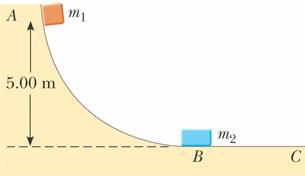
\includegraphics[width=0.4\textwidth]{/home/shluna/UNAHUR/Física/Clases/figs/pistaABC.png}
    %     \caption{ }
    %     \label{fig:pistaABC}
    % \end{figure}

    % \rta $0.56$ m.

    \question Dos bloques, $A$ y $B$, son empujados uno hacia el otro sobre una mesa horizontal lisa. Al principio $B$ está en reposo mientras $A$ se mueve hacia la derecha a $0.5 \, \frac{\un{m}}{\un{s}}$. Después de que chocan, $A$ retrocede a $0.1 \, \frac{\un{m}}{\un{s}}$, mientras que B se mueve a la derecha a $0.3 \, \frac{\un{m}}{\un{s}}$. En un segundo experimento, $A$ está cargado con una masa de $1 \, \un{kg}$ y se le empuja contra $B$ con una velocidad de $0.5 \frac{\un{m}}{\un{s}}$. Después del choque, $A$ queda en reposo y $B$ se mueve hacia la derecha a $0.5 \frac{\un{m}}{\un{s}}$. Hallar la masa de cada bloque.

    \rta $m_A = 1$ kg; $m_B = 2$ kg.

    % \question Las masas de los bloques $A$ y $B$ de la Figura~\ref{fig:bloques} valen $1 \, \un{kg}$ y $2 \, \un{kg}$, respectivamente. Se aprieta uno contra otro, comprimiendo un resorte $S$ colocado entre ellos, y se abandona el sistema partiendo del reposo sobre una superficie horizontal lisa. El resorte no está sujeto a ninguno de los bloques, de modo que cae a la superficie una vez que se ha estirado. El bloque $B$ adquiere una velocidad de $0.5 \frac{\un{m}}{\un{s}}$. ¿Qué energía potencial quedó almacenada en el resorte comprimido?

    % \begin{figure}[h]
    %     \centering
    %     \begin{tikzpicture}[scale=1]
    %         \fill[pattern=north east lines] (0,0) rectangle (7.5,-0.2);
    %         \draw[decoration={coil,segment length = 2mm,amplitude = 2mm,aspect = 0.5,post length = 1mm,pre length = 1mm},decorate,thick,black!50] (2,0.5) -- (5,0.5);
    %         \draw[fill=gray!40] (1,0) rectangle (2,1);
    %         \draw[fill=gray!40] (5,0) rectangle (6.5,1);
    %         \node at (1.5,0.5) {$A$};
    %         \node at (5.75,0.5) {$B$};
    %         \node at (3.5,1) {$S$};
    %         \draw[thick] (0,0) -- (7.5,0);
    %     \end{tikzpicture}
    %     \caption{}
    %     \label{fig:bloques}
    % \end{figure}

    % \rta $0.75$ J.

    \question Un proyectil de masa $m_\text{A} = 50$ g, moviéndose con una rapidez inicial de $500 \, \frac{\text{m}}{\text{s}}$, se dispara hacia un bloque de masa $m_\text{B} = 2$ kg y lo atraviesa, tal como se muestra en la Figura~\ref{fig:bala_bloque_resorte}. El bloque de masa $m_\text{B}$ está unido a un segundo bloque de masa $m_\text{C} = 500$ g mediante un hilo inextensible y de peso despreciable que pasa por una polea de masa también despreciable y sin rozamiento. Al salir, la velocidad del proyectil se reduce a $100 \, \frac{\text{m}}{\text{s}}$, mientras que el bloque se desliza por una superficie horizontal hacia la derecha. El coeficiente de rozamiento entre la superficie y el bloque de masa $m_\text{B}$ es $\mu = 0.25$. Hallar:
    \begin{parts}
        \part La velocidad del bloque de masa $m_\text{B}$ después del choque.
        \part La aceleración del conjunto formado por los dos bloques.
        \part La tensión del hilo que une ambos bloques.
        \part La distancia máxima que alcanza el bloque de masa $m_\text{B}$ a partir del punto $O$.
        \part El tiempo necesario para alcanzar esa distancia máxima y para volver al punto $O$.
    \end{parts}

    \begin{figure}[h]
        \centering
        \begin{subfigure}{0.45\textwidth}
            \centering
            \begin{tikzpicture}[scale=1]
                \fill[pattern=north east lines] (0,-2.5) -- (0.2,-2.5) -- (0.2,-0.2) -- (4.5,-0.2) -- (4.5,0) -- (0,0) -- cycle;
                \draw[fill=gray!40] (1,0) rectangle (2,1);
                \node at (1.5,0.5) {$m_B$};
                \node at (1.5,1.5) {$\vec{v}_{B1} = 0$};
                \draw[thick] (0,-2.5) -- (0,0) -- (4.5,0);
                \fill[black] (1.5,0) circle (0.5mm);
                \node[fill=white] at (1.5,-0.3) {$O$};
                \draw (-0.75,-1.5) -- (-0.75,0.25);
                \draw (-0.5,0.5) -- (1,0.5);
                \draw[thick] (-0.5,0.25) circle (0.25);
                \fill[black] (-0.5,0.25) circle (0.05);
                \draw[ultra thick] (-0.5,0.25) -- (0,0);
                \fill[black] (0.75,0) -- (1,0) -- (1,0.25) --cycle ;
                \draw[fill=gray!40] (-1.05,-2) rectangle (-0.45,-1.2);
                \node at (-0.75,-1.6) {$m_\text{C}$};
                
                \coordinate (A) at (0,0.8);  % To position the bullet in another fig
                \begin{scope}[shift={(A)}, rotate=0,scale=0.1]
                \fill[top color=black!10, bottom color=black!70]
                (0,1) -- (1.5, 1) to [out=0, in=120] (2.5,0.5) to[out=-120, in=0] (1.5,0) -- (0,0) --cycle;
                \draw[white, draw opacity=0.5, line cap=round, line width=0.8mm] (0,0.1) -- (1.5,0.1) to[out=0, in=-140] (2.5,0.5)  (0.02,0) -- (0.02,1) (0.2,0) -- (0.2,1);
                \draw[black!80, line width=0.4mm]   (0,1) -- (1.5, 1) to [out=0, in=120] (2.5,0.5) to[out=-120, in=0] (1.5,0) -- (0,0) --cycle (0.18,0) -- (0.18,1);
                \end{scope}
                \node[anchor=south east] at (-0.2,0.9) {$m_A$};
                \draw (-0.75,0.85) -- (-0.1,0.85);
                \draw (-0.65,0.9) -- (-0.1,0.9);
                \draw (-0.6,0.8) -- (-0.1,0.8);
                \draw[thick,-latex] (-0.25,1.25) -- node[anchor=south]{$\vec{v}_{A1}$} (0.5,1.25);
            \end{tikzpicture}
            \caption{}
            \label{fig:bala_bloque_resorte1}
        \end{subfigure}
        ~
        \begin{subfigure}{0.45\textwidth}
            \centering
            \begin{tikzpicture}[scale=1]
                \fill[pattern=north east lines] (0,-2.5) -- (0.2,-2.5) -- (0.2,-0.2) -- (4.5,-0.2) -- (4.5,0) -- (0,0) -- cycle;
                \draw[fill=gray!40] (1,0) rectangle (2,1);
                \draw[thick] (0,-2.5) -- (0,0) -- (4.5,0);
                \fill[black] (1.5,0) circle (0.5mm);
                \node[fill=white] at (1.5,-0.3) {$O$};
                \draw[fill=gray!40] (-1,-2) rectangle (-0.5,-1.5);
                \draw (-0.75,-1.5) -- (-0.75,0.25);
                \draw (-0.5,0.5) -- (1,0.5);
                \draw[thick] (-0.5,0.25) circle (0.25);
                \fill[black] (-0.5,0.25) circle (0.05);
                \draw[ultra thick] (-0.5,0.25) -- (0,0);
                \fill[black] (0.75,0) -- (1,0) -- (1,0.25) --cycle ;
                \draw[fill=gray!40] (-1.05,-2) rectangle (-0.45,-1.2);
                
                \coordinate (A) at (3,0.8);  % To position the bullet in another fig
                \begin{scope}[shift={(A)}, rotate=0,scale=0.1]
                \fill[top color=black!10, bottom color=black!70]
                (0,1) -- (1.5, 1) to [out=0, in=120] (2.5,0.5) to[out=-120, in=0] (1.5,0) -- (0,0) --cycle;
                \draw[white, draw opacity=0.5, line cap=round, line width=0.8mm] (0,0.1) -- (1.5,0.1) to[out=0, in=-140] (2.5,0.5)  (0.02,0) -- (0.02,1) (0.2,0) -- (0.2,1);
                \draw[black!80, line width=0.4mm]   (0,1) -- (1.5, 1) to [out=0, in=120] (2.5,0.5) to[out=-120, in=0] (1.5,0) -- (0,0) --cycle (0.18,0) -- (0.18,1);
                \end{scope}
                \draw[dashed] (0,0.85) -- (3,0.85);
                \draw[thick,-latex] (2.75,1.25) -- node[anchor=south]{$\vec{v}_{A2}$} (3.5,1.25);
                \draw[thick,-latex] (1.25,1.25) -- node[anchor=south]{$\vec{v}_{B2}$} (2,1.25);
            \end{tikzpicture}
            \caption{}
            \label{fig:bala_bloque_resorte2}
        \end{subfigure}
        \caption{ }
        \label{fig:bala_bloque_resorte}
    \end{figure}

    \rtas
    \begin{enumerate}[a)]
        \item $v_{\text{B}2} = 10 \, \frac{\text{m}}{\text{s}}$.
        \item $a = 3.92 \, \frac{\text{m}}{\text{s}^2}$.
        \item $T = 2.94 \, \text{N}$.
        \item $\Delta x \approx 12.75 \, \text{m}$.
        \item $\Delta t_1 \approx 2.55 \, \text{s}$; $\Delta t_2 \approx 5.1 \, \text{s}$.
    \end{enumerate}

    \section{Momento de inercia y radio de giro}

    \question Una barra de 1 m de longitud tiene ensartados tres bloques de 10 g cada uno como indica la Figura~\ref{fig:Imps}. Calcular el momento de inercia del sistema:
    \begin{parts}
    \part respecto a un eje que pase por un extremo;
    \part respecto a un eje que pase por su centro.
    \end{parts} Despreciar el momento de inercia de la barra.
        
    \begin{figure}[ht]
    \centering
    \begin{tikzpicture}[scale=1]
        \draw[thick] (0,0) -- (6,0);
        \fill[black] (0,0) circle (1mm) node[anchor=south]{10 g};
        \fill[black] (3,0) circle (1mm) node[anchor=south]{10 g};
        \fill[black] (6,0) circle (1mm) node[anchor=south]{10 g};
        \draw (0,-0.2) -- (0,-0.4);
        \draw (3,-0.2) -- (3,-0.4);
        \draw (6,-0.2) -- (6,-0.4);
        \draw[latex-latex] (0,-0.3) -- node[fill=white]{50 cm} (3,-0.3);
        \draw[latex-latex] (3,-0.3) -- node[fill=white]{50 cm} (6,-0.3);
    \end{tikzpicture}
    \caption{ }
    \label{fig:Imps}
    \end{figure}
        
    \begin{solution}
    \begin{parts}
        \part Si el eje pasa por el extremo, 
        \begin{equation*}
        \begin{split}
            I &= \sum_{i=1}^3 m_i \, r_i^2 \\
            &= m_1 \, r_1^2 + m_2 \, r_2^2 + m_3 \, r_3^2 \\
            &= 10 \, \text{g} \times \left(0 \, \text{cm}\right)^2 + 10 \, \text{g} \times \left(50 \, \text{cm}\right)^2 + 10 \, \text{g} \times \left(100 \, \text{cm}\right)^2 \\ 
            &= 125 000 \, \text{g cm}^2
        \end{split}
        \end{equation*}
        \part Si el eje pasa por el medio,
        \begin{equation*}
        \begin{split}
            I &= \sum_{i=1}^3 m_i \, r_i^2 \\
            &= m_1 \, r_1^2 + m_2 \, r_2^2 + m_3 \, r_3^2 \\
            &= 10 \, \text{g} \times \left(50 \, \text{cm}\right)^2 + 10 \, \text{g} \times \left(0 \, \text{cm}\right)^2 + 10 \, \text{g} \times \left(50 \, \text{cm}\right)^2 \\ 
            &= 50 000 \, \text{g cm}^2
        \end{split}
        \end{equation*}
    \end{parts}
    \end{solution}

    \question Una varilla rígida, de longitud $\ell$ y masa despreciable, tiene un masa puntual de $2 \, m$ en su centro y otra masa $m$ en un extremo, pudiendo girar alrededor del otro extremo $O$ (Ver Figura~\ref{fig:varilla}).
    \begin{parts}
        \part Hallar la distancia $x_\text{cm}$ desde $O$ al centro de masa, en función de $\ell$.
        \part Hallar el momento de inercia $I$ del sistema respecto de un eje que pase por $O$ en función de $m$ y de $\ell$.
        \part Calcular el momento de inercia $I_0$, respecto de un eje que pase por el centro de masa en función de $m$ y $\ell$.
        \part Hallar el radio de giro respecto de un eje trazado por $O$ en función de $\ell$.
    \end{parts}

    \begin{figure}[ht]
        \centering
        \begin{tikzpicture}[scale=1]
            \draw[thick] (0,0) node[anchor=south]{$O$} -- node[anchor=south]{$2 \, m$} (6,0) node[anchor=south]{$m$};
            \draw (0,-0.2) -- (0,-0.4) -- (0,-0.8);
            \draw (4,-0.2) -- (4,-0.4);
            \draw (6,-0.2) -- (6,-0.8);
            \draw[latex-latex] (0,-0.3) -- node[fill=white]{$x_\text{cm}$} (4,-0.3);
            \draw[latex-latex] (0,-0.7) -- node[fill=white]{$\ell$} (6,-0.7);
            \fill[black] (0,0) circle (0.5mm);
            \fill[black] (3,0) circle (1mm);
            \fill[black] (6,0) circle (0.8mm);
            \draw[thick] (3.9,-0.1) -- (4.1,0.1);
            \draw[thick] (3.9,0.1) -- (4.1,-0.1);
            \node[anchor=south] at (4,0.1) {CM};
        \end{tikzpicture}
        \caption{ }
        \label{fig:varilla}
    \end{figure}

    \rtas
    \begin{enumerate}[(a)]
        \item $x_\text{cm} = \frac{2 \, \ell}{3}$.
        \item $I = \frac{3}{2} m \, \ell^2$.
        \item $I_0 = \frac{1}{6} m \, \ell^2$. 
        \item $k_0 = \frac{\ell}{\sqrt{2}}$.
    \end{enumerate}

    \question ¿Cuál es el radio de giro de una barra delgada de masa $M$ y longitud $\ell$ respecto a un eje perpendicular a su longitud y que pasa por su punto medio?

    \begin{solution}
    El momento de inercia de una barra respecto a un eje que pasa por su punto medio y es perpendicular a su longitud es $$I = \frac{1}{12} M \, \ell^2$$ Por lo tanto:
    \begin{equation*}
        k = \sqrt{\frac{I}{M}} = \sqrt{\frac{\frac{1}{12} M \, \ell^2}{M}} = \sqrt{\frac{1}{12}} \, \ell = \frac{\ell}{2 \sqrt{3}}
    \end{equation*}
    \end{solution}

    \question El radio interior de un cilindro hueco tiene $7.5$ cm, el exterior, $10$ cm, y su longitud, 15 cm. ¿Cuál es el radio de giro respecto a su eje?

    \rta $8.84$ cm.

    \section{Energía cinética de un cuerpo rígido}

    \question Una rueda de afilar de 15 cm de diámetro, y que tiene una masa de 2 kg, gira a 3600 rpm.
    \begin{parts}
        \part ¿Cuál es su energía cinética de rotación?
        \part ¿De qué altura tendría que caer para adquirir la misma energía cinética?
    \end{parts}

    \rtas
    \begin{enumerate}[(a)]
        \item $E_\text{cr} \approx 400$ J.
        \item $20.41$ m.
    \end{enumerate}

    \section{Dinámica y cinemática del cuerpo rígido}

    \question Una rueda de 30 cm de diámetro gira alrededor de un eje fijo con una velocidad angular inicial de 2 rps. La aceleración es constante e igual a $ 3 \, \frac{\text{rev}}{\text{s}^2}$.
    \begin{parts}
        \part Calcular la velocidad angular al cabo de 6 segundos. Puede asumir que $t_0 = 0$.
        \part ¿Qué ángulo habrá girado la rueda en ese intervalo de tiempo?
        \part ¿Cuál será la velocidad tangencial en un punto de la periferia de la rueda en el instante $t = 6$ s?
        \part ¿Cuánto valen los módulos de las aceleraciones centrípeta y tangencial en $t = 6$ s?
    \end{parts}

    \textbf{Datos:} $1 \, \text{rev} = 2 \, \pi \, \text{rad}$. $1 \, \text{rps} = 1 \, \frac{\text{rev}}{\text{s}} = 1 \, \text{Hz} = 2 \, \pi \, \frac{\text{rad}}{\text{s}}$.

    \rtas
    \begin{enumerate}[(a)]
        \item $\omega = 40 \, \pi \, \frac{\text{rad}}{\text{s}}$.
        \item $\Delta \theta = 132 \, \pi \, \text{rad}$.
        \item $v = 600 \, \pi \, \frac{\text{rad}}{\text{s}}$.
        \item $a_\text{c} = 24000 \, \pi^2 \, \frac{\text{cm}}{\text{s}^2}$; $a_\text{t} = 90 \, \pi \, \frac{\text{cm}}{\text{s}^2}$.
    \end{enumerate}

    \question Una rueda parte del reposo y se acelera uniformemente hasta alcanzar una velocidad angular de 900 rpm en 20 segundos. La distancia del punto al eje es de 15 cm.
    \begin{parts}
        \part Calcular la posición, al cabo de 1 segundo de un punto que se encontraba inicialmente en la parte más alta de la rueda.
        \part Hallar los módulos de las aceleraciones centrípeta y tangencial en dicho instante.
    \end{parts}

    \rtas 
    \begin{enumerate}[(a)]
        \item Gira $135\grado$ a partir del punto más alto.
        \item $a_\text{t} = 71 \, \frac{\text{cm}}{\text{s}^2}$; $a_\text{c} = 333 \, \frac{\text{cm}}{\text{s}^2}$.
    \end{enumerate}

    \question Una rueda de 90 cm de diámetro parte del reposo y va aumentando su velocidad uniformemente hasta alcanzar una velocidad angular de $100 \, \frac{\text{rad}}{\text{s}}$ en 20 segundos. Calcular:
    \begin{parts}
        \part la aceleración angular;
        \part el ángulo girado en ese tiempo.
    \end{parts}

    \rtas
    \begin{enumerate}[(a)]
        \item $5 \, \frac{\text{rad}}{\text{s}^2}$.
        \item 1000 rad.
    \end{enumerate}

    \question La velocidad angular de un volante disminuye uniformemente desde 1000 a 400 rpm, en 5 segundos. Calcular:
    \begin{parts}
        \part la aceleración angular;
        \part el número de revoluciones efectuadas por el volante en el intervalo de 5 segundos.
        \part ¿Cuántos segundos más serán necesarios para que el volante se detenga?
    \end{parts}

    \rtas
    \begin{enumerate}[(a)]
        \item $-4 \, \pi \, \frac{\text{rad}}{\text{s}^2}$.
        \item Unas 58 revoluciones.
        \item 8.33 s.
    \end{enumerate}

    \question Un volante necesita 3 segundos para girar un ángulo de 234 radianes. Su velocidad angular, al cabo de ese tiempo, es $108 \, \frac{\text{rad}}{\text{s}}$. Calcular su aceleración angular, suponiendo que esta es constante.

    \rta $\alpha = 20 \, \frac{\text{rad}}{\text{s}^2}$.

    \question Un volante cuya aceleración angular es constante e igual a $2 \, \dfrac{\text{rad}}{\text{s}^2}$, gira un ángulo de 100 radianes en 5 segundos. ¿Cuánto tiempo ha estado en movimiento antes de comenzar el intervalo de 5 segundos, si partió del reposo?

    \rta $7.5$ s.

    \question Sobre una rueda pivotada se ejerce un momento constante de 20 N m durante un intervalo de tiempo de 10 s, con lo cual la velocidad angular de la rueda aumenta desde cero a 100 rpm. Se suprime entonces el momento exterior, y al cabo de 100 segundos el rozamiento de sus bolilleros hace parar la rueda. Calcular:
    \begin{parts}
        \part El momento de inercia de la rueda.
        \part El momento producido por la fuerza de rozamiento.
        \part El número total de vueltas dado por la rueda.
    \end{parts}

    \rtas
    \begin{enumerate}[(a)]
        \item $19.1 \, \text{kg m}^2$.
        \item $- 2$ N m.
        \item 92 revoluciones.
    \end{enumerate}

    \question Un volante de 400 kg de masa y radio de giro $0.5$ m es acelerado, partiendo del reposo, mediante un motor que desarrolla un momento constante de $\dfrac{200}{\pi}$ N m.
    \begin{parts}
        \part ¿Qué tiempo se requiere para alcanzar una velocidad angular de 600 rpm?
        \part ¿Cuántas revoluciones efectúa el volante en este tiempo?
    \end{parts}

    \rtas
    \begin{enumerate}[(a)]
        \item $10 \, \pi^2$ s.
        \item $100 \, \pi^2$ rad.
    \end{enumerate}

    % \question Los discos $A$ y $B$ de la Figura~\ref{fig:discos} tienen 2 pies de radio y pesan 64 lb, estando rígidamente unidos a los extremos de un eje $C$ que descansa en posición horizontal sobre bolilleros sin rozamiento (no representados). De dos cuerdas arrolladas sobre el borde de cada disco penden dos bloques, uno de 20 lb, unido al disco $A$ y otro de 12 lb, unido al disco $B$, siendo despreciable el momento de inercia de $C$. El sistema parte del reposo.
    % \begin{parts}
    %     \part Hallar la velocidad lineal de cada bloque después que el de 20 lb ha descendido 6 pies.
    %     \part Calcular el momento ejercido por el eje $C$ inmediatamente después de iniciarse el movimiento.
    %     \part Indicar si este momento aumenta, disminuye o permanece constante al proseguir el movimiento.
    % \end{parts}

    % \begin{figure}
    %     \centering
    %     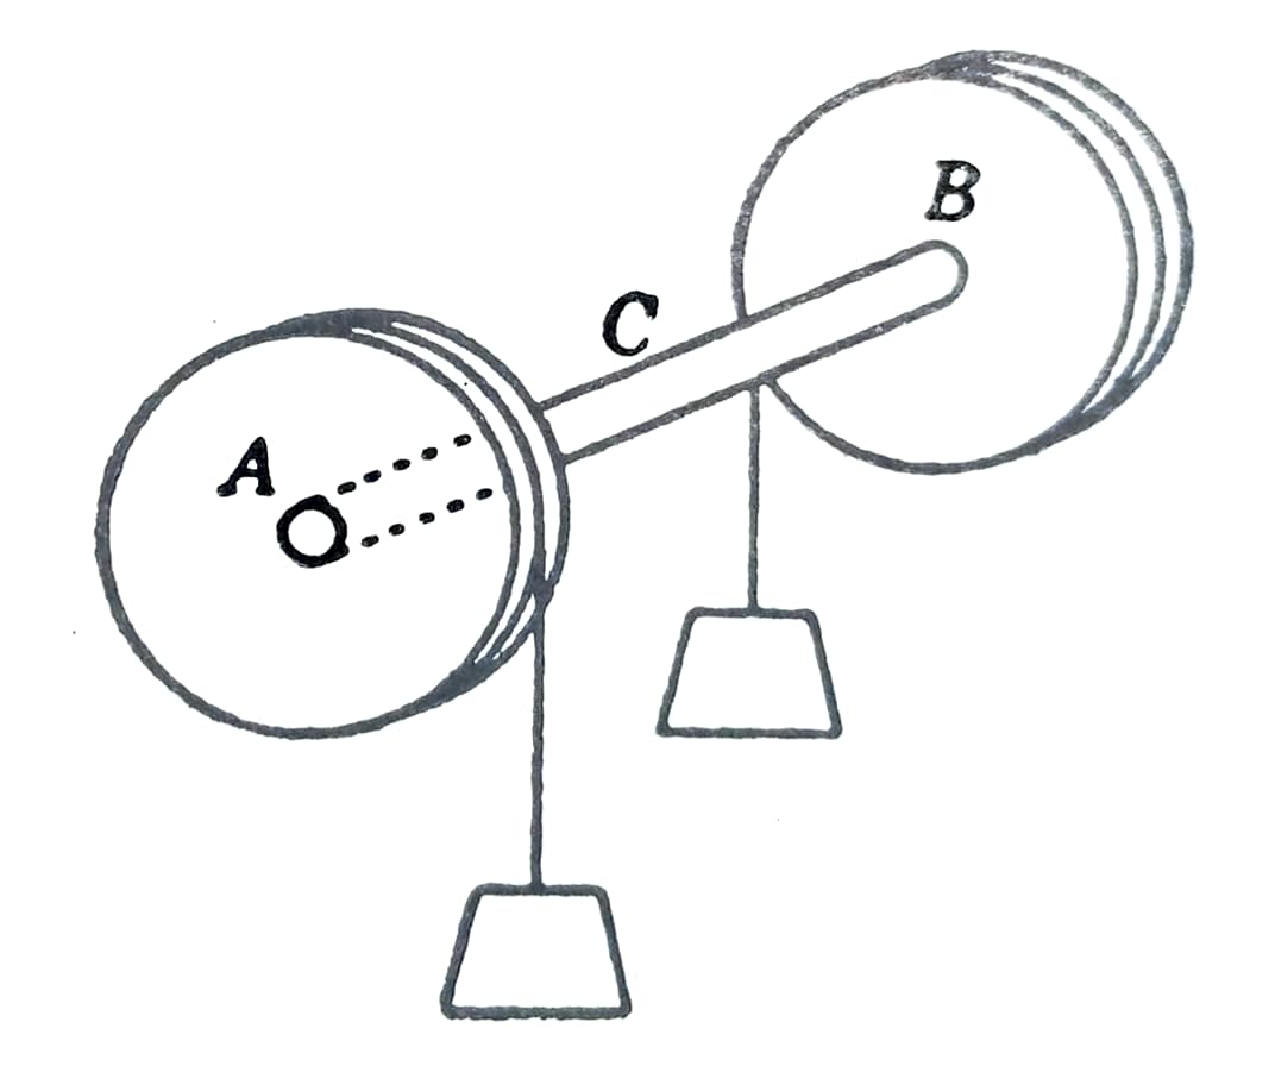
\includegraphics[width=0.3\textwidth]{discos.pdf}
    %     \caption{ }
    %     \label{fig:discos}
    % \end{figure}

    \question De una cuerda arrollada sobre la superficie de un volante de 60 cm de radio pende un bloque de 5 kg de masa (Figura~\ref{fig:volante}). El volante puede girar libremente alrededor de un eje horizontal que pasa por su centro. Calcular su aceleración angular y la tensión de la cuerda, suponiendo igual a $2.94 \, \text{kg m}^2$ el momento de inercia del volante.

    \begin{figure}[ht]
    \centering
    \begin{subfigure}{0.3\textwidth}
        \centering
        \begin{tikzpicture}[scale=1]
        \fill[black] (0,0) circle (0.5mm);
        \draw[thick] (0,0) circle (2);
        \draw[thick] (0,0) -- node[anchor=south]{60 cm} (-2,0);
        \draw[thick] (-2,0) -- (-2,-4);
        \draw[fill=gray!40,thick] (-2.5,-5) rectangle (-1.5,-4);
        \fill[black] (-2,0) circle (0.5mm);
        \end{tikzpicture}
        \caption{ }
        \label{fig:volante}
    \end{subfigure}
    \hfill
    \begin{subfigure}{0.3\textwidth}
        \centering
        \begin{tikzpicture}[scale=1]
            \fill[black] (0,0) circle (0.5mm);
            \draw[thick] (0,0) circle (2);
            \draw[thick] (0,0) -- node[anchor=south]{60 cm} (-2,0);
            \draw[thick,-latex,blue] (-2,0) -- (-2,-2) node[anchor=north]{$\vec{T}$}; 
            \fill[black] (-2,0) circle (0.5mm);
        \end{tikzpicture}
        \caption{ }
        \label{fig:dclvol}
    \end{subfigure}
    \hfill
    \begin{subfigure}{0.3\textwidth}
        \centering
        \begin{tikzpicture}[scale=1]
            \draw[fill=gray!40,thick] (-0.5,-0.5) rectangle (0.5,0.5);
            \draw[thick,red,-latex] (0,0) -- (0,-3) node[anchor=west]{$\vec{F}_\text{g}$};
            \draw[thick,blue,-latex] (0,0) -- (0,2) node[anchor=west]{$\vec{T}$};
            \fill[black] (0,0) circle (0.5mm);
        \end{tikzpicture}
        \caption{ }
        \label{fig:dclbloque}
    \end{subfigure}
    \caption{ }
    \label{fig:volantebloque}
    \end{figure}

    \begin{solution}
    Los diagramas de fuerzas correspondientes al volante y al bloque aislados se dan en las Figuras~\ref{fig:dclvol} y \ref{fig:dclbloque}, respectivamente. Se han omitido las fuerzas en el centro del volante debido a que es nulo su momento respecto al eje de rotación.

    A partir de la Figura~\ref{fig:dclvol} podemos observar que la tensión $\vec{T}$ de la cuerda produce un torque que hace girar el volante en sentido antihorario. La componente $z$ de dicho torque es: $$\tau = T \, R$$ donde $R$ es el radio del volante. En virtud de la ecuación de movimiento del sólido rígido, tenemos que:
    \begin{equation*}
        \begin{split}
            \tau &= I \, \alpha \\
        T \, R &= I \, \alpha
        \end{split}
    \end{equation*} Por otro lado, las fuerzas que actúan sobre el bloque son la tensión $\vec{T}$ de la cuerda y el peso $\vec{F}_\text{g}$ del bloque. Las componentes de estas fuerzas son:
    \begin{align*}
        \vec{T} &= \left(0;T\right) \\
        \vec{F}_\text{g} &= \left(0;-m \, g\right).
    \end{align*} Por lo tanto, la suma de las fuerzas en la dirección vertical da: $$\sum f_y = T - m \, g = - m \, a_y$$ Esta suma es distinta de cero por que el bloque no se encuentra suspendido en equilibrio sino que baja con una cierta aceleración que debemos determinar. Para ello, debemos tener en cuenta que el módulo de la aceleración lineal del bloque debe ser igual al módulo de la aceleración tangencial del volante: $$a_y = a_\text{t} = R \, \alpha$$ Así, obtenemos un sistema de tres ecuaciones que vinculan las tres incógnitas del problema ($T$, $\alpha$ y $a_y$) con los datos dados en el enunciado:
    \begin{align}
        T \, R &= I \, \alpha \label{ec:volante} \\
        T - m \, g &= - m \, a_y  \label{ec:bloque} \\
        a_y &= R \, \alpha  \label{ec:at}
    \end{align} Teniendo en cuenta la tercera ecuación, podemos reescribir la segundo como: $$T = m \, g - m \, R \, \alpha $$ Esta expresión del módulo de la tensión se puede reemplazar en la Ecuación~\eqref{ec:volante} para obtener: $$\left(m \, g - m \, R \, \alpha\right) R = I \, \alpha ,$$ de donde se puede despejar la aceleración angular: $$\alpha = \frac{m \, g \, R}{I + m \, R^2}$$ Esta última expresión se puede reemplazar en la Ecuación~\eqref{ec:at} para obtener: $$a_y = \frac{m \, g \, R^2}{I + m \, R^2} = g \left(\frac{1}{1 + \frac{I}{m \, R^2}}\right)$$ de donde se concluye que el bloque desciende con una aceleración menor que la de la gravedad debido a la resistencia que ofrece el volante a la aceleración angular producida por el torque aplicado sobre él.

    Reemplazando los valores correspondientes en las expresiones de $\alpha$, $a_y$ y $T$, obtenemos:
    \begin{align*}
        \alpha &= 6.20 \, \frac{\text{rad}}{\text{s}^2} \\
        a_y &= 3.72 \, \frac{\text{m}}{\text{s}^2} \\
            T &= 30.38 \, \text{N}
    \end{align*}

    Podemos demostrar de forma analítica que la pérdida (o variación) de energía potencial gravitatoria del bloque es igual a la suma de los incrementos de energía cinética del bloque y de energía cinética de rotación del volante.

    Cuando el bloque descienda una altura $\Delta y$ la correspondiente variación de energía potencial gravitatoria será $$\Delta E_\text{pg} = m \, g \, \Delta y$$ Como el bloque está unido al volante mediante una cuerda, la variación de altura será igual a la longitud de arco correspondiente al desplazamiento angular del volante: $$\Delta y = \Delta s = R \, \Delta \theta$$ Por lo tanto, $$\Delta E_\text{pg} = m \, g \, R \, \Delta \theta$$ Por otro lado, la variación de energía cinética del bloque sumada a la variación de energía cinética de rotación del volante es: 
    \begin{equation*}
        \begin{split}
        \Delta E_\text{c} + \Delta E_\text{cr} &= \left(\frac{1}{2} m \, v^2 - \frac{1}{2} m \, v_0^2\right) + \left(\frac{1}{2} I \, \omega^2 - \frac{1}{2} I \, \omega_0^2\right) \\
        &= \frac{1}{2} m \left(v^2 - v_0^2\right) + \frac{1}{2} I \left(\omega^2 - \omega_0^2\right)
        \end{split}
    \end{equation*} Ahora bien, tenemos que $$v^2 = v_0^2 + 2 \, a_y \, \Delta y$$ donde, como vimos, $a_y = a_\text{t} = R \, \alpha$ y $\Delta y = R \, \Delta \theta$, en consecuencia: $$v^2 - v_0^2 = 2 \left(R \, \alpha\right) \left(R \, \Delta \theta\right) = 2 \, R^2 \, \alpha \, \Delta \theta$$ Además: $$\omega^2 = \omega_0^2 + 2 \, \alpha \, \Delta \theta$$ O bien: $$\omega^2 - \omega_0^2 = 2 \, \alpha \, \Delta \theta$$ Luego:
    \begin{equation*}
        \begin{split}
        \Delta E_\text{c} + \Delta E_\text{cr} &= \frac{1}{2} m \left(v^2 - v_0^2\right) + \frac{1}{2} I \left(\omega^2 - \omega_0^2\right) \\
        &= \frac{1}{2} m \left(2 \, R^2 \, \alpha \, \Delta \theta\right) + \frac{1}{2} I \left(2 \, \alpha \, \Delta \theta\right) \\
        &= \left(m \, R^2 + I\right) \alpha \, \Delta \theta
        \end{split}
    \end{equation*} Como $$\alpha = \frac{m \, g \, R}{I + m \, R^2},$$ entonces: $$ \Delta E_\text{c} + \Delta E_\text{cr} = \left(m \, R^2 + I\right) \frac{m \, g \, R}{\left(I + m \, R^2\right)} \, \Delta \theta = \cancel{\left(m \, R^2 + I\right)} \frac{m \, g \, R}{\cancel{\left(I + m \, R^2\right)}} \, \Delta \theta = m \, g \, R \, \Delta \theta = \Delta E_\text{pg}$$
    \end{solution}

    \question En la llanta de un volante de 60 cm de radio está arrollada una cuerda sobre la que se ejerce una fuerza constante de 49 N, como indica la Figura~\ref{fig:volante}. El volante está montado sobre bolilleros sin rozamiento en un eje horizontal que pasa por su centro y su momento de inercia es de $0.098 \, \text{kg m}^2$. 
    \begin{parts}
        \part Calcular la aceleración angular del volante.
        \part Probar que el trabajo realizado para desenrollar 6 m de cuerda equivale, aproximadamente, al incremento de energía cinética de la rueda.
        \part Si, como muestra la Figura~\ref{fig:dclvol} se cuelga un bloque de 5 kg de masa de la cuerda, ¿cuál sera su aceleración angular? ¿Por qué no es la misma que en el caso (a)?
    \end{parts}

    % \begin{figure}[h]
    % \centering
    % \begin{subfigure}{0.45\textwidth}
    %     \centering
    %     \begin{tikzpicture}[scale=1]
    %         \fill[black] (0,0) circle (0.5mm);
    %         \draw[thick] (0,0) circle (2);
    %         \draw[thick] (0,0) -- node[anchor=south]{60 cm} (-2,0);
    %         \draw[thick,-latex,blue] (-2,0) -- (-2,-2) node[anchor=north]{$\vec{F}$}; 
    %         \fill[black] (-2,0) circle (0.5mm);
    %     \end{tikzpicture}
    %     \caption{ }
    %     \label{fig:volante}
    % \end{subfigure}
    % \hfill
    % \begin{subfigure}{0.45\textwidth}
    %     \centering
    %     \begin{tikzpicture}[scale=1]
    %         \fill[black] (0,0) circle (0.5mm);
    %         \draw[thick] (0,0) circle (2);
    %         \draw[thick] (0,0) -- node[anchor=south]{60 cm} (-2,0);
    %         \draw[thick] (-2,0) -- (-2,-4);
    %         \draw[fill=gray!40,thick] (-2.5,-5) rectangle (-1.5,-4);
    %         \fill[black] (-2,0) circle (0.5mm);
    %     \end{tikzpicture}
    %     \caption{ }
    %     \label{fig:dclvol}
    % \end{subfigure}
    % \caption{ }
    % \label{fig:volantebloque}
    % \end{figure}

    \rtas
    \begin{enumerate}[(a)]
        \item $300 \, \frac{\text{rad}}{\text{s}^2}$.
        \item $W = \Delta E_\text{cr} = 294$ J.
        \item $15.49 \, \frac{\text{rad}}{\text{s}^2}$.
    \end{enumerate}

    \question Un cubo de agua que tiene una masa de 32 kg está suspendido de una cuerda arrollada alrededor de un torno que tiene la forma de un cilindro macizo de 30 cm de diámetro y que tiene también una masa de 32 kg (Figura~\ref{fig:cubo}). El cubo se deja caer, partiendo del reposo, desde la boca de un pozo y desciende una altura de 20 m antes de llegar al agua.
    \begin{parts}
        \part ¿Cuál es la tensión de la cuerda mientras cae el cubo?
        \part ¿Con qué velocidad llega el cubo al agua?
        \part ¿Cuánto tarda en caer? 
    \end{parts} Desprecie el peso de la cuerda.

    \begin{figure}[ht]
        \centering
        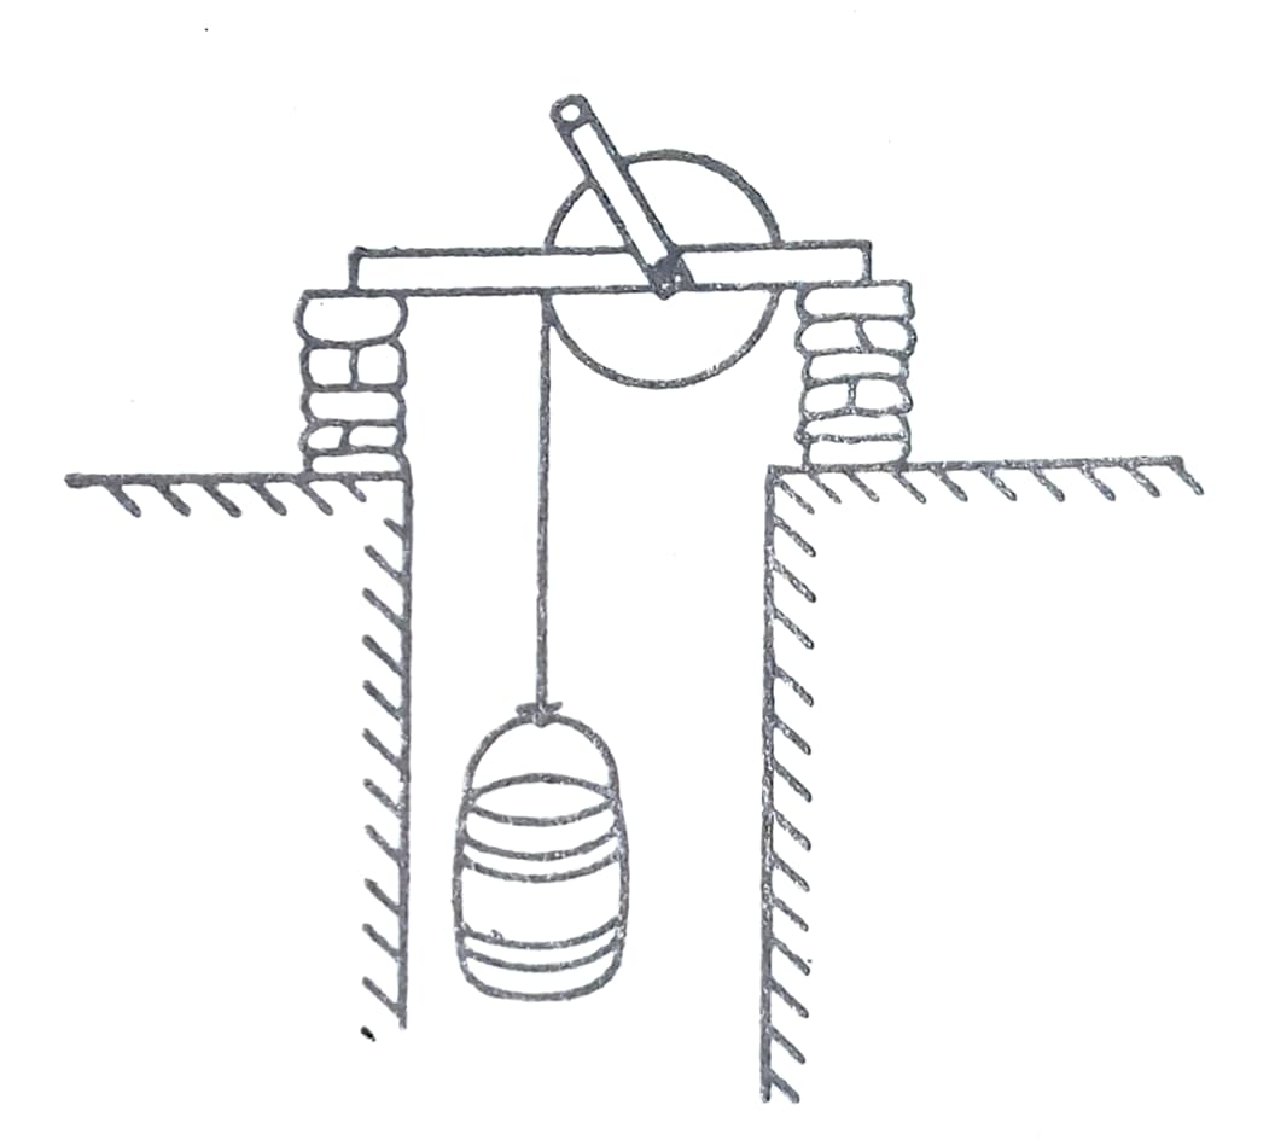
\includegraphics[width=0.3\textwidth]{//home/shluna/Proyectos/Clases_Fisica_III/figs/cubo.pdf}
        \caption{ }
        \label{fig:cubo}
    \end{figure}

    \rtas
    \begin{enumerate}[(a)]
        \item $104.53$ N.
        \item $16.17 \, \frac{\text{m}}{\text{s}}$.
        \item $2.47$ s.
    \end{enumerate}

    \question Un bloque de masa $m = 5$ kg desliza por la superficie de un plano inclinado $37\grado$ según se indica en la Figura~\ref{fig:planoincvol}. El coeficiente cinético de rozamiento es $0.25$. Una cuerda unida al bloque pasa por la llanta de un volante de eje $O$. La masa del volante es $M = 20$ kg.
    \begin{parts}
        \part ¿Con qué aceleración desciende el bloque por el plano?
        \part ¿Cuál es la tensión en la cuerda?
    \end{parts}

    \begin{figure}[ht]
        \centering
        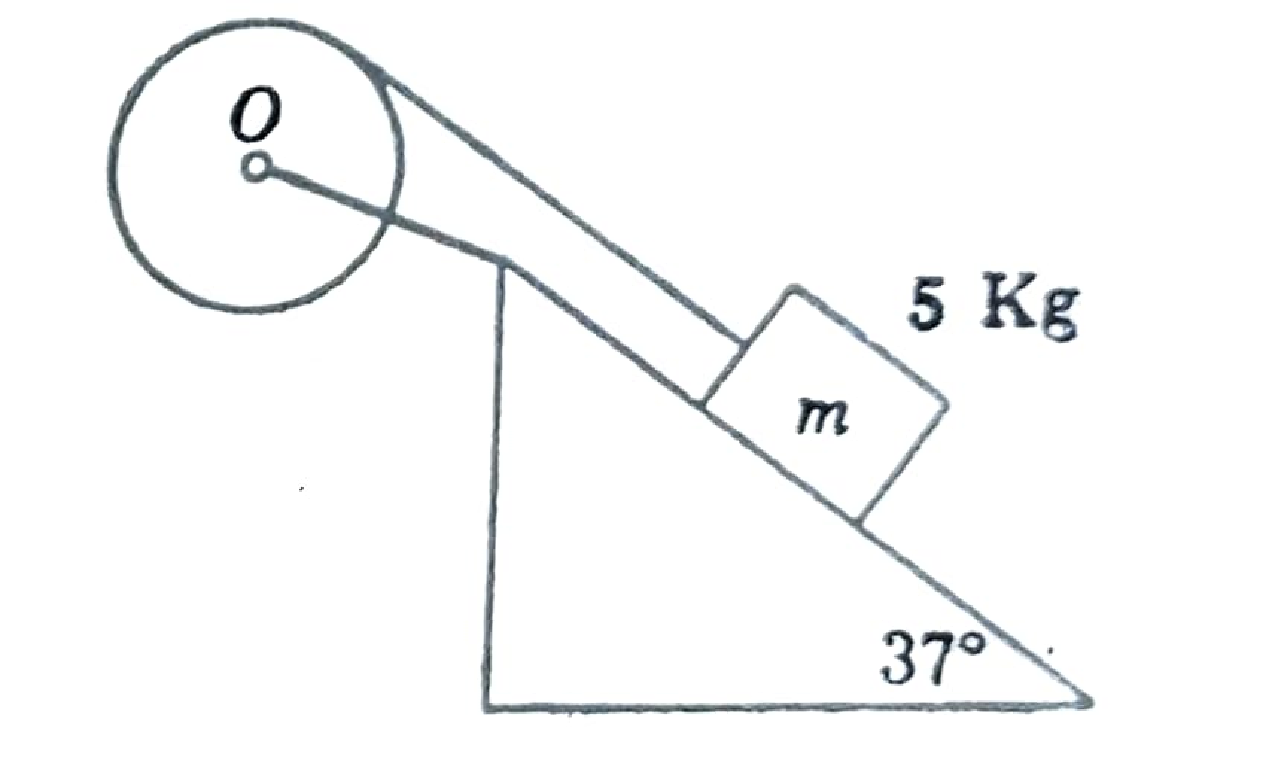
\includegraphics[width=0.3\textwidth]{/home/shluna/Proyectos/Clases_Fisica_III/figs/planoincvolante.pdf}
        \caption{ }
        \label{fig:planoincvol}
    \end{figure}

    \rtas
    \begin{enumerate}[(a)]
        \item $1.31 \, \frac{\text{m}}{\text{s}^2}$.
        \item $13.14 \, \text{N}$.
    \end{enumerate}

    \question Un bloque de 8 kg de masa se encuentra en reposo sobre una superficie horizontal lisa. Una cuerda atada al bloque pasa por una polea, cuyo diámetro tiene 15 cm, y en el otro extremo de la cuerda cuelga otro bloque cuya masa es también de 8 kg. Se abandona el sistema desde el reposo y se observa que el bloque recorre 5 m en 2 s.
    \begin{parts}
        \part ¿Cuál es el momento de inercia de la polea?
        \part ¿Cuál es la tensión en cada parte de la cuerda?
    \end{parts}

    \section{Conservación del momento angular}

    \question Una persona que se encuentra de pie en el centro de una plataforma giratoria, tiene sus brazos extendidos horizontalmente, con una masa de 5 kg en cada mano. Se le pone en rotación alrededor de un eje vertical con una velocidad angular de una vuelta cada 2 segundos. Calcular su nueva velocidad angular si deja caer sus manos a ambos lados del cuerpo. El momento de inercia de la persona puede suponerse constante e igual a $c$. La distancia inicial de las masas al eje ($r_0$) es de 90 cm y su distancia final ($r$) es de 15 cm.

    \begin{solution}
    Si es despreciable el rozamiento de la plataforma giratoria, no se ejerce ningún momento exterior al sistema respecto al eje vertical y el momento angular del sistema se conserva. Esto es: $$L = L_0$$ donde $L$ es el valor final del momento de inercia y $L_0$ es su valor inicial. Como $L = I \, \omega$: $$I \, \omega = \left(I \omega\right)_0 = I_0 \, \omega_0$$ donde, ahora, $\omega$ y $\omega_0$ son los valores final e inicial de la velocidad angular, mientras que $I$ e $I_0$ son los valores final e inicial del momento de inercia. El momento de inercia del sistema formado por la persona y por las dos masas (que pueden considerarse puntuales) es igual a la suma de los momentos de inercia de cada parte, es decir: $$I = I_\text{persona} + I_\text{masas puntuales}$$ donde $\, \Delta \theta = 5.88 \, \text{kg m}^2$ e $I_\text{masas puntuales} = 2 \, m \, r^2$. En consecuencia:
    \begin{align*}
        I &= I_\text{persona} + 2 \, m \, r^2 = 5.88 \, \text{kg m}^2 + 2 \time 5 \, \text{kg} \times (0.15 \, \text{m})^2 = 6.11 \, \text{kg m}^2 \\
        I_0 &= I_\text{persona} + 2 \, m \, r_0^2 = 5.88 \, \text{kg m}^2 + 2 \time 5 \, \text{kg} \times (0.90 \, \text{m})^2 = 13.98 \, \text{kg m}^2 
    \end{align*} Por otro lado, la velocidad angular inicial es $$\omega_0 = \frac{1 \, \text{vuelta}}{2 \, \text{s}} = \frac{2 \, \pi \, \text{rad}}{2 \, \text{s}} = \pi \, \frac{\text{rad}}{\text{s}}$$ Luego, despejando la velocidad angular final de la expresión de la conservación del momento angular, se obtiene: $$\omega = \omega_0 \frac{I_0}{I} = 2.29 \, \frac{\text{rad}}{\text{s}}$$ Es decir, cuando la persona baja las manos, su velocidad angular aumenta un poco más del doble.
    \end{solution}

    \section{Torque de la resultante y centro de gravedad}

    \question Determinar la intensidad y línea de acción de la resultante de las tres fuerzas de la Figura~\ref{fig:paralelas}.

    \begin{figure}[ht]
    \centering
    \begin{tikzpicture}[scale=1]
        \draw[ultra thick] (0,0) -- (6,0);
        \fill[black] (1.5,0) circle (1mm);
        \node[anchor=south] at (1.5,0) {$O$};
        \fill[black] (0,0) circle (1mm);
        \node[anchor=east] at (0,0) {$P$};
        \draw[thick,-latex,blue] (0,0) -- (0,1) node[anchor=south] {19.6 N};
        \draw[thick,-latex,blue] (2.5,0) -- (2.5,-3) node[anchor=north] {98 N};
        \draw[thick,-latex,blue] (6,0) -- (6,2) node[anchor=south] {29.4 N};
        \draw[thick] (0,-0.2) -- (0,-0.6);
        \draw[thick] (1.5,-0.2) -- (1.5,-0.6);
        \draw[thick] (6,-0.2) -- (6,-0.6);
        \draw[thick,latex-latex] (0,-0.4) -- node[fill=white]{3 m} (1.5,-0.4);
        \draw[thick,latex-latex] (1.5,-0.4) -- node[anchor=north]{2 m} (2.5,-0.4);
        \draw[thick,latex-latex] (2.5,-0.4) -- node[fill=white]{4 m} (6,-0.4);
    \end{tikzpicture}
    \caption{ }
    \label{fig:paralelas}
    \end{figure}

    \begin{solution}
    Consideremos primero un eje perpendicular al plano de la Figura~\ref{fig:paralelas} que pase por el punto $O$. Entonces: $$x = \frac{19.6 \, \text{N} \times (-3 \, \text{m}) + (-98 \, \text{N}) \times 2 \, \text{m} + 29.4 \, \text{N} \times 6 \, \text{m}}{19.6 \, \text{N} - 98 \, \text{N} + 29.4 \, \text{N}} = \frac{-78.4 \, \text{N m}}{-49 \, \text{N}} = 1.6 \, \text{m}$$

    Si hubiésemos considerado el punto $P$, tendríamos: $$x = \frac{19.6 \, \text{N} \times 0 + (-98 \, \text{N}) \times 5 \, \text{m} + 29.4 \, \text{N} \times 9 \, \text{m}}{19.6 \, \text{N} - 98 \, \text{N} + 29.4 \, \text{N}} = \frac{-225.4 \, \text{N m}}{-49 \, \text{N}} = 4.6 \, \text{m}$$
    \end{solution}

    \question Hallar la posición del centro de gravedad de los tres pesos de la Figura~\ref{fig:cdg}.

    \begin{figure}[ht]
    \centering
    \begin{tikzpicture}[scale=1]
        \draw[thick] (-2,0) -- (2,0);
        \draw[thick] (0,0) -- (0,3);
        \fill[black] (-2,0) circle (0.5mm);
        \fill[black] (2,0) circle (0.5mm);
        \fill[black] (0,3) circle (0.5mm);
        \fill[black] (0,0) circle (0.5mm);
        \node[anchor=north] at (0,0) {$O$};
        \node[anchor=north] at (-2,0) {$m_1 = 4 \, \text{kg}$};
        \node[anchor=north] at (2,0) {$m_2 = 4 \, \text{kg}$};
        \node[anchor=south] at (0,3) {$m_3 = 16 \, \text{kg}$};
        \draw[thick] (-2,0.2) -- (-2,0.6);
        \draw[thick] (2,0.2) -- (2,0.6);
        \draw[thick] (-0.3,3) -- (-0.7,3);
        \draw[thick,latex-latex] (-2,0.4) -- node[fill=white]{2 m} (0,0.4);
        \draw[thick,latex-latex] (0,0.4) -- node[fill=white]{2 m} (2,0.4);
        \draw[thick,latex-latex] (-0.5,0) -- node[fill=white]{3 m} (-0.5,3);
        \fill[red] (0,2) circle (0.5mm) node[anchor=west]{CG};
    \end{tikzpicture}
    \caption{ }
    \label{fig:cdg}
    \end{figure}

    \begin{solution}
    Si consideramos un sistema de referencia cartesiano, cuyo origen coincida con el punto $O$ de la Figura~\ref{fig:cdg}, tendremos:
    \begin{itemize}
        \item $F_{g}^{(1)} = m_1 \, g = 4 \, \text{kg} \times 9.8 \, \dfrac{\text{m}}{\text{s}^2} = 39.2 \, \text{N}$; $x_1 = - 2 \, \text{m}$, $y_1 = 0$.
        \item $F_{g}^{(2)} = m_2 \, g = 4 \, \text{kg} \times 9.8 \, \dfrac{\text{m}}{\text{s}^2} = 39.2 \, \text{N}$; $x_2 = 2 \, \text{m}$, $y_2 = 0$.
        \item $F_{g}^{(3)} = m_3 \, g = 16 \, \text{kg} \times 9.8 \, \dfrac{\text{m}}{\text{s}^2} = 156.8 \, \text{N}$; $x_3 = 0$, $y_3 = 3 \, \text{m}$.
    \end{itemize} Luego: $$\bar{x} = \frac{F_{g}^{(1)} \, x_1 + F_{g}^{(2)} \, x_2 + F_{g}^{(3)} \, x_3}{F_{g}^{(1)} + F_{g}^{(2)} + F_{g}^{(3)}} = \frac{39.2 \, \text{N} \times (-2 \, \text{m}) + 39.2 \, \text{N} \times 2 \, \text{m} + 156.8 \, \text{N} \times 0 \, \text{m}}{39.2 \, \text{N} + 39.2 \, \text{N} + 156.8 \, \text{N}} = 0 \, \text{m}$$ $$\bar{y} = \frac{F_{g}^{(1)} \, y_1 + F_{g}^{(2)} \, y_2 + F_{g}^{(3)} \, y_3}{F_{g}^{(1)} + F_{g}^{(2)} + F_{g}^{(3)}} = \frac{39.2 \, \text{N} \times 0 \, \text{m} + 39.2 \, \text{N} \times 0 \, \text{m} + 156.8 \, \text{N} \times 3 \, \text{m}}{39.2 \, \text{N} + 39.2 \, \text{N} + 156.8 \, \text{N}} = 2 \, \text{m}$$
    \end{solution}

    \section{Segunda condición de equilibrio}

    \question Un niño de \( 21 \, \text{kg} \) de masa se sienta en un subibaja a \( 2 \, \text{m}\) del centro de giro \( O \), donde se encuentra el soporte (Figura~\ref{fig:subibaja}). 

    \begin{parts}
    \part ¿A qué distancia \( d \) del centro de giro deberá sentarse, al otro lado, su padre, que tiene una masa de \( 105 \, \text{kg}\) para que el subibaja se encuentre en equilibrio?
    \part ¿Cuánto vale el módulo de la fuerza \( \mathbf{F} \) que el soporte ejerce sobre el subibaja?
    \end{parts}

    \begin{figure}[ht]
    \centering
    \begin{tikzpicture}[scale=1]
        \fill[pattern=north east lines] (-0.5,-0.5) rectangle (0.5,-0.7);
        \draw[thick] (-0.5,-0.5) -- (0.5,-0.5) -- (0,0) -- cycle;
        \draw[ultra thick] (-4.5,0) -- (4.5,0);
        \draw[latex-latex] (-2,0.5) -- node[fill=white]{$d$} (0,0.5);
        \draw (-2,0.3) -- (-2,0.7);
        \draw[latex-latex] (0,0.5) -- node[fill=white]{$2 \, \text{m}$} (4,0.5);
        \draw (4,0.3) -- (4,0.7);
        \draw[thick,red,-latex] (0,0) -- (0,2) node[anchor=west]{$\vec{F}$};
        \draw[thick,blue,-latex] (4,0) -- (4,-2) node[anchor=west]{$\vec{F}_\text{g, Niño}$};
        \draw[thick,blue,-latex] (-2,0) -- (-2,-2) node[anchor=west]{$\vec{F}_\text{g, Padre}$};
        \fill[black] (0,0) circle (0.5mm) node[anchor=south west]{$O$};
    \end{tikzpicture}
    \caption{ }
    \label{fig:subibaja}
    \end{figure}

    \begin{solution}
    A fin de evitar que el subibaja gire, se debe cumplir la segunda condición de equilibrio, es decir, que la suma de los momentos de las fuerzas sea igual a cero. Si tomamos como origen del sistema de referencia al punto de giro \( O \) del subibaja, entonces tenemos que $$ \sum \tau^{O} = P_\text{Padre} \cdot d - P_\text{Niño} \cdot 2 \, \text{m} = 0 $$ El segundo término del lado izquierdo puede pasarse sumando al lado derecho: $$ P_\text{Padre} \cdot d = P_\text{Niño} \cdot 2 \, \text{m} $$ Luego, se puede despejar la distancia \( d \): $$ d = \frac{P_\text{Niño} \cdot 2 \, \text{m}}{P_\text{Padre}}$$ Ahora bien, tenemos además que \( P_\text{Padre} = m_\text{Padre} \cdot g \) y que \( P_\text{Niño} = m_\text{Niño} \cdot g \). Entonces: $$d = \frac{m_\text{Niño} \cdot g \cdot 2 \, \text{m}}{m_\text{Padre} \cdot g} = \frac{m_\text{Niño} \cdot 2 \, \text{m}}{m_\text{Padre}} $$ Reemplazando los valores \( m_\text{Niño} = 21 \, \text{kg} \) y \( m_\text{Padre} = 105 \, \text{kg} \), obtenemos: $$d = \frac{21 \, \text{kg} \cdot 2 \, \text{m}}{105 \, \text{kg}} = 0.4 \text{m} $$

    Para determinar la fuerza que el soporte ejerce sobre el subibaja, debemos plantear la primera condición de equilibrio. Como las fuerzas solamente tienen dirección vertical, entonces es suficiente sumar las fuerzas en esa dirección (\( y \)): $$ \sum f_y = F - P_\text{padre} - P_\text{Niño} = 0$$ Luego: $$F = P_\text{padre} + P_\text{Niño} = m_\text{Padre} \cdot g + m_\text{Niño} \cdot g  = \left(m_\text{Padre} + m_\text{Niño}\right) \cdot g $$ Reemplazando los valores correspondientes, se obtiene: $$F = \left( 105 \, \text{kg} + 21 \, \text{kg}\right) \cdot 9.8 \frac{\text{m}}{\text{s}} = 1234.8 \, \text{N} $$
    \end{solution}

    \question Una balanza se encuentra suspendida por un cable delgado cuya masa es despreciable. La balanza consiste en una varilla rígida de masa también despreciable, de la que cuelga en su extremo izquierdo un bloque \( A \) de \( 3 \, \text{kg} \) a  \( 20 \, \text{cm} \) del punto donde la balanza se une con el cable que la sostiene, tal como se muestra en la Figura~\ref{fig:balanza}. 

    \begin{parts}
        \part ¿A qué distancia \( x \) a la derecha de dicho punto se debe suspender una bloque de \( B \) de \( 2 \, \text{kg} \) para que el sistema se encuentre en equilibrio estático? 
        \part ¿Cuánto vale la tensión \( T \) del  cable?
    \end{parts}

    \begin{figure}[ht]
        \centering
        \begin{tikzpicture}[scale=1]
            \draw[ultra thick] (-2,0) -- (4.5,0);
            \node[anchor=north] at (0,0) {$O$};
            \draw[thick] (0,0) -- (0,2);
            \fill[pattern=north east lines] (-0.5,2) -- (0.5,2) -- (0.5,2.2) -- (-0.5,2.2) -- cycle;
            \draw[thick] (-0.5,2) -- (0.5,2);
            \draw[thick] (-2,0) -- (-2,-1);
            \draw[thick] (4,0) -- (4,-1);
            \draw[fill=gray!40] (-2.5,-2) rectangle (-1.5,-1);
            \draw[fill=gray!40] (3.7,-1.5) rectangle (4.3,-1);
            \node at (-2,-1.5) {$A$};
            \node at (4,-1.25) {$B$};
            \draw[thick,latex-latex] (-2,0.5) -- node[fill=white]{20 cm} (0,0.5);
            \draw[thick,latex-latex] (0,0.5) -- node[fill=white]{$x$} (4,0.5);
            \draw[thick] (-2,0.3) -- (-2,0.7);
            \draw[thick] (4,0.3) -- (4,0.7);
        \end{tikzpicture}
        \caption{}
        \label{fig:balanza}
    \end{figure}

    \rtas \(x = 0.3 \, \text{m} \);  \( T = 49 \, \text{N} \).

    \question Para mantener en equilibrio, en la posición representada, la barra de la Figura~\ref{fig:barraybloques} ha de aplicarse una sola fuerza, $\vec{F}$. La masa del bloque $A$ es de 5 kg y la masa del bloque $B$ es de 2 kg. Pueden despreciarse el peso de la barra y las masas de las cuerdas.
    \begin{parts}
    \part ¿Cuáles son las componentes $x$ e $y$ de la fuerza requerida?
    \part ¿Cuál es el módulo de la fuerza requerida y el ángulo, $\varphi$, que forma su dirección con el eje de los $x$ positivos?
    \part ¿Dónde debe aplicarse dicha fuerza?
    \end{parts}

    \begin{figure}[ht]
    \centering
    \begin{tikzpicture}[scale=1]
        \fill[black] (0,0) circle (0.5mm);
        \draw[thick] (-1,0) -- (0,0);
        \fill[pattern=north east lines] (-1,-0.5) -- (-1,0.5) -- (-1.2,0.5) -- (-1.2,-0.5) -- cycle;
        \draw[thick] (-1,-0.5) -- (-1,0.5);
        \draw[thick] (0,0) -- (60:2);
        \draw[fill=gray!40,thick] ({2*cos(60)},{2*sin(60)-0.1}) rectangle ({2*cos(60)+6},{2*sin(60)+0.1});
        \draw[thick,latex-latex] ({2*cos(60)},{2*sin(60)-0.5}) -- node[fill=white]{3 m} ({2*cos(60)+6},{2*sin(60)-0.5});
        \fill[black] (60:2) circle (0.5mm);
        \draw[dashed] (60:2) -- ({2*cos(60)},0);
        \draw[thick] (0,0) -- (0,-1);
        \draw[fill=gray!40,thick] (-0.5,-2) rectangle (0.5,-1);
        \draw[thick] ({2*cos(60)+6},{2*sin(60)}) -- ({2*cos(60)+6},{2*sin(60)-2});
        \draw[fill=gray!40,thick] ({2*cos(60)+6-0.25},{2*sin(60)-2.5}) rectangle ({2*cos(60)+6+0.25},{2*sin(60)-2});
        \node at (0,-1.5) {$A$};
        \node at ({2*cos(60)+6},{2*sin(60)-2.25}) {$B$};
        \draw[thick] ({2*cos(60)},{2*sin(60)-1}) arc (270:240:1);
        \node at ({2*cos(60)-0.3},0.5) {$30\grado$};
        \draw[thick,red,-latex] ({2*cos(60)+4},{2*sin(60)}) -- node[anchor=south east]{$\vec{F}$} ({2*cos(60)+4+2*cos(60)},{2*sin(60)+2*sin(60)});
        \draw[red] ({2*cos(60)+4.5},{2*sin(60)}) arc (0:60:0.5);
        \draw[thick,red,latex-latex] ({2*cos(60)},{2*sin(60)+0.5}) -- node[fill=white]{$d$} ({2*cos(60)+4},{2*sin(60)+0.5});
        \draw[thick,red] ({2*cos(60)},{2*sin(60)+0.3}) -- ({2*cos(60)},{2*sin(60)+0.7});
        \draw[thick,red] ({2*cos(60)+4},{2*sin(60)+0.3}) -- ({2*cos(60)+4},{2*sin(60)+0.7});
        \node[anchor=south west,red] at ({2*cos(60)+4+0.5*cos(30)},{2*sin(60)+0.5*sin(30)}) {$\varphi$};
        \node[anchor=east] at ({2*cos(60)},{2*sin(60)}) {$O$};
    \end{tikzpicture}
    \caption{ }
    \label{fig:barraybloques}
    \end{figure}

    \rtas
    \begin{enumerate}[(a)]
        \item $F_x = 28.29$ N; $F_y = 68.6$ N.
        \item $F = 74.20$ N; $\varphi = \angulo{67}{35}{21.14}$.
        \item $d = 0.86$ m, es decir, a 86 cm a la derecha del punto $O$.
    \end{enumerate}

    \question Determinar los módulos de las tensiones de las cuerdas $A$ y $B$ en la Figuras~\ref{fig:barraconpeso} y las componentes de la fuerza que el perno $O$, de manera que el sistema permanezca en equilibrio estático. Despreciar la masa de las cuerdas. La masa del bloque es de $80 \, \un{kg}$ y la de la barra es de $40 \, \un{kg}$.

    \begin{figure}[ht]
    \centering
    \begin{subfigure}{0.45\textwidth}
        \centering
        \begin{tikzpicture}[scale=1]
        \fill[pattern=north east lines] (-0.2,-2.5) -- (0,-2.5) -- (0,4.5) -- (-0.2,4.5) -- cycle;
        \draw[thick] (0,-2.5) -- (0,4.5);
        \draw[ultra thick] (0,0) -- (4,0);
        \draw[thick,fill=white] (0,-0.2) arc (-90:90:0.2);
        \draw[fill=black] (0,0) circle (0.5mm);
        \draw[fill=black] (0,4) circle (0.5mm);
        \draw[fill=black] (4,0) circle (0.5mm);
        \draw[thick] (0,4) -- node[anchor=south west]{$A$} (4,0) -- node[anchor=west]{$B$} (4,-1);
        \draw[fill=gray!40] (3.5,-2) rectangle (4.5,-1);
        \node[anchor=south] at (3.2,0) {$45\grado$};
        \node[anchor=south west] at (0.1,0.1) {$O$};
        \draw[thick,latex-latex] (0,-0.5) -- node[fill=white]{$L$} (4,-0.5);
    \end{tikzpicture}
    \caption{}
    \label{fig:barraconpeso}
    \end{subfigure}
    ~
    \begin{subfigure}{0.45\textwidth}
        \centering
        \begin{tikzpicture}[scale=1]
        \draw[thick,-latex] (0,0) -- (4.5,0) node[anchor=north]{$x$};
        \draw[thick,-latex] (0,-2.5) -- (0,2.5) node[anchor=east]{$y$};
        \draw[ultra thick] (0,0) -- (4,0);
        \draw[fill=black] (0,0) circle (0.5mm);
        \node[anchor=south east] at (0,0) {$O$};
        \draw[thick,latex-latex] (0,-1.5) -- node[fill=white]{$L$} (4,-1.5);
        \draw[thick,-latex,blue] (-1,0) node[anchor=south]{$F_x$} -- (0,0);
        \draw[thick,-latex,blue] (0,-1) node[anchor=east]{$F_y$} -- (0,0);
        \draw[fill=black] (4,0) circle (0.5mm);
        \draw[thick,-latex,green] (4,0) -- node[anchor=south west]{$\vec{T}$} (2.5,1.5);
        \node[anchor=south,green] at (3.2,0) {$45\grado$};
        \draw[thick,-latex,green] (4,0) -- node[anchor=north]{$T_x$} (2.5,0);
        \draw[thick,-latex,green] (4,0) -- node[anchor=west]{$T_y$} (4,1.5);
        \draw[dashed,green] (2.5,0) -- (2.5,1.5) -- (4,1.5);
        \draw[thick,-latex,red] (4,0) -- (4,-2) node[anchor=west]{$\vec{F}_\text{g, bloque}$};
        \draw[thick,-latex,red] (2,0) -- (2,-1) node[anchor=west]{$\vec{F}_\text{g, barra}$};
        \end{tikzpicture}
        \caption{ }
        \label{fig:dcl}
    \end{subfigure}
    \caption{ }
    \label{fig:barraconpeso2}
    \end{figure}

    \begin{solution}
    Consideremos un sistema de referencia cartesiano cuyo origen coincide con el punto $O$, donde se encuentra el perno, tal como se muestra en la Figura~\ref{fig:dcl}. Las componentes de los vectores $\vec{T}$, $\vec{F}$, $\vec{F}_\text{g,barra}$ y $\vec{F}_\text{g,bloque}$ en dicho sistema de referencia son:
    \begin{itemize}
        \item $\vec{T} = \left(-T_x;T_y\right)$.
        \item $\vec{F} = \left(F_x;F_y\right)$.
        \item $\vec{F}_\text{g, barra} = \left(0;-m_\text{barra} \, g\right)$.
        \item $\vec{F}_\text{g, bloque} = \left(0;-m_\text{bloque} \, g\right)$.
    \end{itemize} El siguiente paso es plantear las dos condiciones de equilibrio:
    \begin{align}
        \sum f_x &= F_x - T_x = 0 \label{ec:sumx} \\
        \sum f_y &= F_y + T_y - m_\text{barra} \, g -m_\text{bloque} \, g = 0 \label{ec:sumy} \\
        \sum \tau^{O} &= T_y \, L - m_\text{barra} \, g \, \frac{L}{2} -m_\text{bloque} \, g \, L = 0 \label{ec:sumt} 
    \end{align} De la Ecuación~\eqref{ec:sumt} podemos despejar $T_y$: $$T_y = \frac{\left(m_\text{bloque} + \frac{m_\text{barra}}{2}\right) g\, L}{L} = \left(m_\text{bloque} + \frac{m_\text{barra}}{2}\right) g$$ Luego: $$T_y = \left(80 \, \text{kg} + \frac{40 \, \text{kg}}{2}\right) \times 9.8 \, \frac{\text{m}}{\text{s}^2} = 980 \, \text{N}$$

    Una vez determinado el valor de $T_y$, podemos usarlo para hallar el valor de $F_y$ en virtud de la Ecuación~\eqref{ec:sumy}: $$F_y = \left(m_\text{bloque} + m_\text{barra} g - T_y\right) = \left(80 \, \text{kg} + 40 \, \text{kg}\right) \times 9.8 \, \frac{\text{m}}{\text{s}^2} - 980 \, \text{N} = 196 \, \text{N}$$ Por último, de la Ecuación~\eqref{ec:sumx} se obtiene: $$F_x = T_x$$ Las componentes horizontal y vertical de la tensión están relacionadas mediante: $$\frac{T_y}{T_x} = \tan 45\grado = 1$$ y, por lo tanto: $$T_x = T_y = 980 \, \text{N}$$ En consecuencia, $$F_x = T_x = 980 \, \text{N}$$
    \end{solution}

    \question Hallar la el módulo de la tensión ($T$) del cable $BD$ de la Figura~\ref{fig:puntal} y las componentes horizontal ($F_x$) y vertical ($F_y$) de la fuerza ejercida sobre el el puntal $AB$ por el perno $A$. La masa del bloque es de 10 kg.

    \begin{figure}[ht]
        \centering
        \begin{tikzpicture}[scale=1]
            \fill[pattern=north east lines] (-0.2,-2.5) -- (0,-2.5) -- (0,2.5) -- (-0.2,2.5) -- cycle;
            \draw[thick] (0,-2.5) -- (0,2.5);
            \draw[ultra thick] (0,0) -- (4,0);
            \draw[thick,fill=white] (0,-0.2) arc (-90:90:0.2);
            \draw[fill=black] (0,0) circle (0.5mm);
            \draw[fill=black] (0,2) circle (0.5mm);
            \draw[fill=black] (4,0) circle (0.5mm);
            \draw[thick] (0,2) -- (4,0);
            \draw[thick] (3,0) -- (3,-1);
            \fill[black] (3,0) circle (0.5mm);
            \draw[fill=gray!40] (2.5,-2) rectangle (3.5,-1);
            \draw[latex-latex] (0,-0.4) -- node[anchor=north]{90 cm} (3,-0.4);
            \draw[latex-latex] (3,-0.4) -- node[anchor=north]{30 cm} (4,-0.4);
            \draw (4,-0.6) -- (4,-0.2);
            \draw[latex-latex] (-0.5,0) -- node[anchor=east]{90 cm} (-0.5,2);
            \draw (-0.7,0) -- (-0.3,0);
            \draw (-0.7,2) -- (-0.3,2);
            \node[anchor=south west] at (0,2) {$D$};
            \node[anchor=south west] at (0.1,0.1) {$A$};
            \node[anchor=south west] at (4,0) {$B$};
            \node[anchor=south] at (3,0) {$C$};
        \end{tikzpicture}
        \caption{ }
        \label{fig:puntal}
    \end{figure}

    \rtas $T = 122.5$ N; $F_x = 98$ N; $F_y = 24.5$ N.

    \question Hallar nuevamente el módulo de la tensión ($T$) del cable $BD$ de la Figura~\ref{fig:puntal} y las componentes horizontal ($F_x$) y vertical ($F_y$) de la fuerza ejercida sobre el el puntal $AB$ por el perno $A$, pero esta vez considerando que la masa del bloque es de 40 kg y que la masa de la barra es de 10 kg.

    \rtas $T = 408.34$ N, $F_x = 326.67$ N y $F_y = 245$ N.

\end{questions}

    \begin{table}[ht]
        \centering
        \begin{tabular}{|c|cccccccccc|}
            \hline
            $\alpha$ (grados)   & $0\grado$ &  $30\grado$ & $45\grado$ & $60\grado$ & $90\grado$ & $135\grado$ & $180\grado$ & $225\grado$ & $270\grado$ & $315\grado$ \\
            \hline
            $\alpha$ (radianes) &   $0$    &  $\frac{\pi}{6}$ & $\frac{\pi}{4}$ & $\frac{\pi}{3}$ & $\frac{\pi}{2}$ & $\frac{3}{4} \pi$ & $\pi$ & $\frac{5}{4} \pi$ & $\frac{3}{2} \pi$ & $\frac{7}{4} \pi$ \\
            \hline
            $\sin \alpha$       &   $0$    & $\frac{1}{2}$ & $\frac{\sqrt{2}}{2}$ & $\frac{\sqrt{3}}{2}$ & $1$ & $\frac{\sqrt{2}}{2}$ & $0$ & $\frac{-\sqrt{2}}{2}$ & $-1$ & $-\frac{\sqrt{2}}{2}$ \\
            $\cos \alpha$       &   $1$    & $\frac{\sqrt{3}}{2}$ & $\frac{\sqrt{2}}{2}$ & $\frac{1}{2}$ & $0$ & $-\frac{\sqrt{2}}{2}$ & $-1$ & $-\frac{\sqrt{2}}{2}$ & $0$ & $\frac{\sqrt{2}}{2}$ \\
            $\tan \alpha$       &   $0$    & $\frac{\sqrt{3}}{3}$ & $1$ & $\sqrt{3}$ & $+\infty$ & $-1$ & $0$ & $1$ & $-\infty$ & $-1$ \\
            \hline  
        \end{tabular}
    \end{table}

\end{document}